\documentclass{beamer}
\usetheme{metropolis}
\usepackage{tikz}
\usepackage[none]{hyphenat}
\usepackage{fontawesome}
\usepackage{pifont}
\input{epigraph.tex}

\title{Keynesians to the Rescue: Unprecedented Policy Responses Towards Unprecedented Macroeconomic Shocks (Evidence from Three Natural Experiments)}
\subtitle{Lille Post-Keynesian Conference 
\newline December 6-8, 2023 }
\date{Dec 6, 2023}
\author{Lyuben Ivanov, PhD}
\institute{Faculty of Economics and Business, Sofia University St. Kliment Ohridski}

\begin{document}

\maketitle

\section{Introduction}

\begin{frame}{Research Background}
\vfill
\begin{list}{\faChevronCircleRight}{\leftmargin=3.4em \labelsep=1.5em 
\itemsep = 1.5em}
\item Inspired by a series of columns from Barry Eichengreen and Kevin O'Rourke in Vox.eu which shattered readership records in 2009 (\textit{A Tale of Two Depressions}) started on Apr 6, 2009
\item Inspired by a column by Paul Krugman in New York Times (\textit{The Great Recession versus the Great Depression}) published on Mar 20, 2009
\item Inspired by an article in New York Times (\textit{Rapid Declines in Manufacturing Spread Global Anxiety}) published on Mar 20, 2009
\end{list}
	
\end{frame}

\begin{frame}{Research Outline}
Part I. Fiscal and monetary responses to three major macroeconomic shocks
\begin{list}{\faChevronCircleRight}{\leftmargin=3.4em \labelsep=1.5em 
\itemsep = 1em}
\item [\ding{202}] Fiscal response in USA and the Euro Area (EA) to the Great Depression of 1929 (baseline scenario), the 2007-2009 Global Financial and Economic Crisis (a.k.a the Great Recession)
\item [\ding{203}] Fiscal response in USA and the Euro Area (EA) to the Great Depression of 1929 (baseline scenario), the 2007-2009 Global Financial and Economic Crisis (a.k.a the Great Recession)
\end{list}
\end{frame}

\begin{frame}{Research Outline}
Part II. Macroeconomic outcomes
\begin{list}{\faChevronCircleRight}{\leftmargin=3.4em \labelsep=1.5em 
\itemsep = 1em}
\item [\ding{202}] Industrial production in USA and the EA (EA) during the Great Recession and post the COVID-19 pandemic
\item [\ding{203}] Employment in USA and the EA (EA) during the Great Recession and post the COVID-19 pandemic
\item [\ding{204}] Stock markets in USA and the EA (EA) during the Great Recession and post the COVID-19 pandemic

\end{list}	
\end{frame}


\section{Fiscal and Monetary Responses to Three Major Macroeconomic Shocks}

\begin{frame}{Fiscal Response to the GFC and the COVID-19 Pandemic}

\begin{figure}[h!]
     \centering
     % Created by tikzDevice version 0.12.5 on 2023-11-24 22:28:42
% !TEX encoding = UTF-8 Unicode
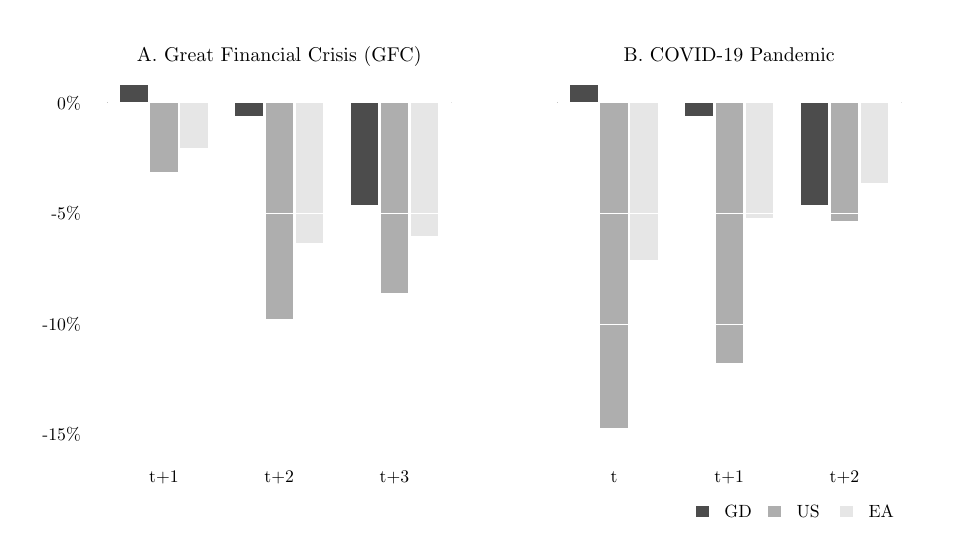
\begin{tikzpicture}[x=1pt,y=1pt]
\definecolor{fillColor}{RGB}{255,255,255}
\path[use as bounding box,fill=fillColor,fill opacity=0.00] (0,0) rectangle (325.21,180.67);
\begin{scope}
\path[clip] (  0.00,  0.00) rectangle (162.61,180.67);
\definecolor{fillColor}{gray}{0.30}

\path[fill=fillColor] ( 33.40,153.48) rectangle ( 43.31,159.88);
\definecolor{fillColor}{RGB}{174,174,174}

\path[fill=fillColor] ( 44.31,153.48) rectangle ( 54.22,128.67);
\definecolor{fillColor}{RGB}{230,230,230}

\path[fill=fillColor] ( 55.21,153.48) rectangle ( 65.13,137.14);
\definecolor{fillColor}{gray}{0.30}

\path[fill=fillColor] ( 75.04,153.48) rectangle ( 84.96,148.71);
\definecolor{fillColor}{RGB}{174,174,174}

\path[fill=fillColor] ( 85.95,153.48) rectangle ( 95.86, 75.50);
\definecolor{fillColor}{RGB}{230,230,230}

\path[fill=fillColor] ( 96.85,153.48) rectangle (106.77,102.79);
\definecolor{fillColor}{gray}{0.30}

\path[fill=fillColor] (116.68,153.48) rectangle (126.60,116.76);
\definecolor{fillColor}{RGB}{174,174,174}

\path[fill=fillColor] (127.59,153.48) rectangle (137.50, 84.74);
\definecolor{fillColor}{RGB}{230,230,230}

\path[fill=fillColor] (138.49,153.48) rectangle (148.41,105.51);
\end{scope}
\begin{scope}
\path[clip] (  0.00,  0.00) rectangle (325.21,180.67);
\definecolor{drawColor}{RGB}{0,0,0}

\node[text=drawColor,anchor=base,inner sep=0pt, outer sep=0pt, scale=  0.64] at ( 49.26, 16.32) {t+1};

\node[text=drawColor,anchor=base,inner sep=0pt, outer sep=0pt, scale=  0.64] at ( 90.90, 16.32) {t+2};

\node[text=drawColor,anchor=base,inner sep=0pt, outer sep=0pt, scale=  0.64] at (132.54, 16.32) {t+3};
\end{scope}
\begin{scope}
\path[clip] ( 28.80, 33.60) rectangle (153.01,161.47);
\definecolor{drawColor}{RGB}{0,0,0}

\path[draw=drawColor,line width= 0.4pt,line join=round,line cap=round] ( 28.80,153.48) -- (153.01,153.48);
\end{scope}
\begin{scope}
\path[clip] (  0.00,  0.00) rectangle (325.21,180.67);
\definecolor{drawColor}{RGB}{0,0,0}

\node[text=drawColor,anchor=base east,inner sep=0pt, outer sep=0pt, scale=  0.64] at ( 19.20, 31.40) {-15\%};

\node[text=drawColor,anchor=base east,inner sep=0pt, outer sep=0pt, scale=  0.64] at ( 19.20, 71.36) {-10\%};

\node[text=drawColor,anchor=base east,inner sep=0pt, outer sep=0pt, scale=  0.64] at ( 19.20,111.32) {-5\%};

\node[text=drawColor,anchor=base east,inner sep=0pt, outer sep=0pt, scale=  0.64] at ( 19.20,151.28) {0\%};
\end{scope}
\begin{scope}
\path[clip] ( 28.80, 33.60) rectangle (153.01,161.47);
\definecolor{drawColor}{RGB}{255,255,255}

\path[draw=drawColor,line width= 0.4pt,line join=round,line cap=round] ( 28.80, 33.60) -- (153.01, 33.60);

\path[draw=drawColor,line width= 0.4pt,line join=round,line cap=round] ( 28.80, 73.56) -- (153.01, 73.56);

\path[draw=drawColor,line width= 0.4pt,line join=round,line cap=round] ( 28.80,113.52) -- (153.01,113.52);

\path[draw=drawColor,line width= 0.4pt,line join=round,line cap=round] ( 28.80,153.48) -- (153.01,153.48);
\end{scope}
\begin{scope}
\path[clip] (  0.00,  0.00) rectangle (162.61,180.67);
\definecolor{drawColor}{RGB}{0,0,0}

\node[text=drawColor,anchor=base,inner sep=0pt, outer sep=0pt, scale=  0.72] at ( 90.90,168.60) {A. Great Financial Crisis (GFC)};
\end{scope}
\begin{scope}
\path[clip] (162.61,  0.00) rectangle (325.21,180.67);
\definecolor{fillColor}{gray}{0.30}

\path[fill=fillColor] (196.01,153.48) rectangle (205.92,159.88);
\definecolor{fillColor}{RGB}{174,174,174}

\path[fill=fillColor] (206.91,153.48) rectangle (216.83, 36.07);
\definecolor{fillColor}{RGB}{230,230,230}

\path[fill=fillColor] (217.82,153.48) rectangle (227.73, 96.74);
\definecolor{fillColor}{gray}{0.30}

\path[fill=fillColor] (237.65,153.48) rectangle (247.56,148.71);
\definecolor{fillColor}{RGB}{174,174,174}

\path[fill=fillColor] (248.55,153.48) rectangle (258.47, 59.47);
\definecolor{fillColor}{RGB}{230,230,230}

\path[fill=fillColor] (259.46,153.48) rectangle (269.37,111.92);
\definecolor{fillColor}{gray}{0.30}

\path[fill=fillColor] (279.29,153.48) rectangle (289.20,116.76);
\definecolor{fillColor}{RGB}{174,174,174}

\path[fill=fillColor] (290.19,153.48) rectangle (300.11,110.78);
\definecolor{fillColor}{RGB}{230,230,230}

\path[fill=fillColor] (301.10,153.48) rectangle (311.01,124.71);
\end{scope}
\begin{scope}
\path[clip] (  0.00,  0.00) rectangle (325.21,180.67);
\definecolor{drawColor}{RGB}{0,0,0}

\node[text=drawColor,anchor=base,inner sep=0pt, outer sep=0pt, scale=  0.64] at (211.87, 16.32) {t};

\node[text=drawColor,anchor=base,inner sep=0pt, outer sep=0pt, scale=  0.64] at (253.51, 16.32) {t+1};

\node[text=drawColor,anchor=base,inner sep=0pt, outer sep=0pt, scale=  0.64] at (295.15, 16.32) {t+2};
\end{scope}
\begin{scope}
\path[clip] (191.41, 33.60) rectangle (315.62,161.47);
\definecolor{drawColor}{RGB}{0,0,0}

\path[draw=drawColor,line width= 0.4pt,line join=round,line cap=round] (191.41,153.48) -- (315.62,153.48);
\definecolor{drawColor}{RGB}{255,255,255}

\path[draw=drawColor,line width= 0.4pt,line join=round,line cap=round] (191.41, 33.60) -- (315.62, 33.60);

\path[draw=drawColor,line width= 0.4pt,line join=round,line cap=round] (191.41, 73.56) -- (315.62, 73.56);

\path[draw=drawColor,line width= 0.4pt,line join=round,line cap=round] (191.41,113.52) -- (315.62,113.52);

\path[draw=drawColor,line width= 0.4pt,line join=round,line cap=round] (191.41,153.48) -- (315.62,153.48);
\end{scope}
\begin{scope}
\path[clip] (162.61,  0.00) rectangle (325.21,180.67);
\definecolor{fillColor}{gray}{0.30}

\path[fill=fillColor] (241.43,  7.86) rectangle (246.03,  4.02);
\definecolor{fillColor}{RGB}{174,174,174}

\path[fill=fillColor] (267.46,  7.86) rectangle (272.07,  4.02);
\definecolor{fillColor}{RGB}{230,230,230}

\path[fill=fillColor] (293.50,  7.86) rectangle (298.11,  4.02);
\definecolor{drawColor}{RGB}{0,0,0}

\node[text=drawColor,anchor=base west,inner sep=0pt, outer sep=0pt, scale=  0.64] at (251.79,  3.74) {GD};

\node[text=drawColor,anchor=base west,inner sep=0pt, outer sep=0pt, scale=  0.64] at (277.83,  3.74) {US};

\node[text=drawColor,anchor=base west,inner sep=0pt, outer sep=0pt, scale=  0.64] at (303.87,  3.74) {EA};

\node[text=drawColor,anchor=base,inner sep=0pt, outer sep=0pt, scale=  0.72] at (253.51,168.60) {B. COVID-19 Pandemic};
\end{scope}
\end{tikzpicture}

\end{figure} 
	
\end{frame}

\begin{frame}{Monetary Response to the GFC and the COVID-19 Pandemic}

\begin{figure}[h!]
     \centering
     % Created by tikzDevice version 0.12.5 on 2023-11-24 22:28:42
% !TEX encoding = UTF-8 Unicode
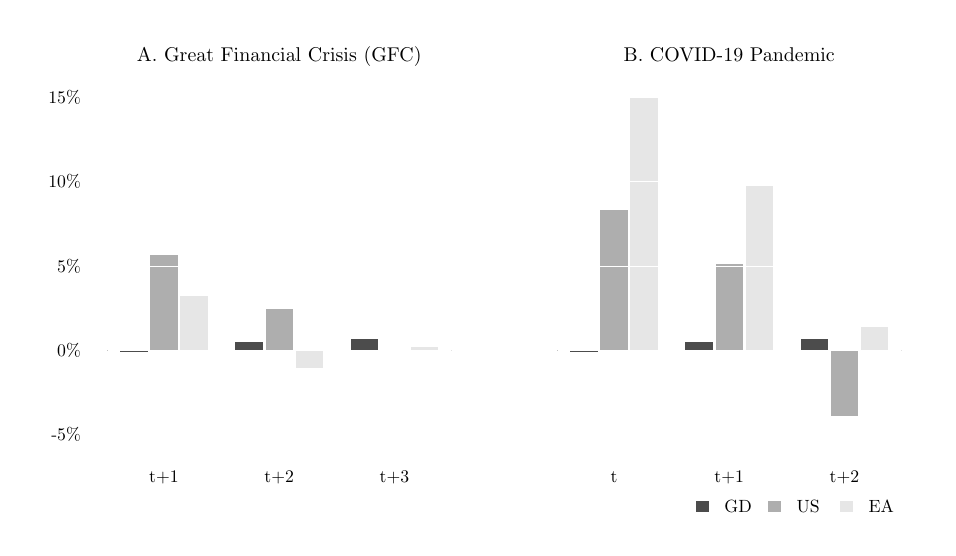
\begin{tikzpicture}[x=1pt,y=1pt]
\definecolor{fillColor}{RGB}{255,255,255}
\path[use as bounding box,fill=fillColor,fill opacity=0.00] (0,0) rectangle (325.21,180.67);
\begin{scope}
\path[clip] (  0.00,  0.00) rectangle (162.61,180.67);
\definecolor{fillColor}{gray}{0.30}

\path[fill=fillColor] ( 33.40, 64.05) rectangle ( 43.31, 63.46);
\definecolor{fillColor}{RGB}{174,174,174}

\path[fill=fillColor] ( 44.31, 64.05) rectangle ( 54.22, 98.40);
\definecolor{fillColor}{RGB}{230,230,230}

\path[fill=fillColor] ( 55.21, 64.05) rectangle ( 65.13, 83.59);
\definecolor{fillColor}{gray}{0.30}

\path[fill=fillColor] ( 75.04, 64.05) rectangle ( 84.96, 67.13);
\definecolor{fillColor}{RGB}{174,174,174}

\path[fill=fillColor] ( 85.95, 64.05) rectangle ( 95.86, 78.89);
\definecolor{fillColor}{RGB}{230,230,230}

\path[fill=fillColor] ( 96.85, 64.05) rectangle (106.77, 57.59);
\definecolor{fillColor}{gray}{0.30}

\path[fill=fillColor] (116.68, 64.05) rectangle (126.60, 68.16);
\definecolor{fillColor}{RGB}{174,174,174}

\path[fill=fillColor] (127.59, 64.05) rectangle (137.50, 63.72);
\definecolor{fillColor}{RGB}{230,230,230}

\path[fill=fillColor] (138.49, 64.05) rectangle (148.41, 65.37);
\end{scope}
\begin{scope}
\path[clip] (  0.00,  0.00) rectangle (325.21,180.67);
\definecolor{drawColor}{RGB}{0,0,0}

\node[text=drawColor,anchor=base,inner sep=0pt, outer sep=0pt, scale=  0.64] at ( 49.26, 16.32) {t+1};

\node[text=drawColor,anchor=base,inner sep=0pt, outer sep=0pt, scale=  0.64] at ( 90.90, 16.32) {t+2};

\node[text=drawColor,anchor=base,inner sep=0pt, outer sep=0pt, scale=  0.64] at (132.54, 16.32) {t+3};
\end{scope}
\begin{scope}
\path[clip] ( 28.80, 33.60) rectangle (153.01,161.47);
\definecolor{drawColor}{RGB}{0,0,0}

\path[draw=drawColor,line width= 0.4pt,line join=round,line cap=round] ( 28.80, 64.05) -- (153.01, 64.05);
\end{scope}
\begin{scope}
\path[clip] (  0.00,  0.00) rectangle (325.21,180.67);
\definecolor{drawColor}{RGB}{0,0,0}

\node[text=drawColor,anchor=base east,inner sep=0pt, outer sep=0pt, scale=  0.64] at ( 19.20, 31.40) {-5\%};

\node[text=drawColor,anchor=base east,inner sep=0pt, outer sep=0pt, scale=  0.64] at ( 19.20, 61.84) {0\%};

\node[text=drawColor,anchor=base east,inner sep=0pt, outer sep=0pt, scale=  0.64] at ( 19.20, 92.29) {5\%};

\node[text=drawColor,anchor=base east,inner sep=0pt, outer sep=0pt, scale=  0.64] at ( 19.20,122.74) {10\%};

\node[text=drawColor,anchor=base east,inner sep=0pt, outer sep=0pt, scale=  0.64] at ( 19.20,153.18) {15\%};
\end{scope}
\begin{scope}
\path[clip] ( 28.80, 33.60) rectangle (153.01,161.47);
\definecolor{drawColor}{RGB}{255,255,255}

\path[draw=drawColor,line width= 0.4pt,line join=round,line cap=round] ( 28.80, 33.60) -- (153.01, 33.60);

\path[draw=drawColor,line width= 0.4pt,line join=round,line cap=round] ( 28.80, 64.05) -- (153.01, 64.05);

\path[draw=drawColor,line width= 0.4pt,line join=round,line cap=round] ( 28.80, 94.49) -- (153.01, 94.49);

\path[draw=drawColor,line width= 0.4pt,line join=round,line cap=round] ( 28.80,124.94) -- (153.01,124.94);

\path[draw=drawColor,line width= 0.4pt,line join=round,line cap=round] ( 28.80,155.39) -- (153.01,155.39);
\end{scope}
\begin{scope}
\path[clip] (  0.00,  0.00) rectangle (162.61,180.67);
\definecolor{drawColor}{RGB}{0,0,0}

\node[text=drawColor,anchor=base,inner sep=0pt, outer sep=0pt, scale=  0.72] at ( 90.90,168.60) {A. Great Financial Crisis (GFC)};
\end{scope}
\begin{scope}
\path[clip] (162.61,  0.00) rectangle (325.21,180.67);
\definecolor{fillColor}{gray}{0.30}

\path[fill=fillColor] (196.01, 64.05) rectangle (205.92, 63.46);
\definecolor{fillColor}{RGB}{174,174,174}

\path[fill=fillColor] (206.91, 64.05) rectangle (216.83,114.88);
\definecolor{fillColor}{RGB}{230,230,230}

\path[fill=fillColor] (217.82, 64.05) rectangle (227.73,155.23);
\definecolor{fillColor}{gray}{0.30}

\path[fill=fillColor] (237.65, 64.05) rectangle (247.56, 67.13);
\definecolor{fillColor}{RGB}{174,174,174}

\path[fill=fillColor] (248.55, 64.05) rectangle (258.47, 95.19);
\definecolor{fillColor}{RGB}{230,230,230}

\path[fill=fillColor] (259.46, 64.05) rectangle (269.37,123.37);
\definecolor{fillColor}{gray}{0.30}

\path[fill=fillColor] (279.29, 64.05) rectangle (289.20, 68.16);
\definecolor{fillColor}{RGB}{174,174,174}

\path[fill=fillColor] (290.19, 64.05) rectangle (300.11, 40.23);
\definecolor{fillColor}{RGB}{230,230,230}

\path[fill=fillColor] (301.10, 64.05) rectangle (311.01, 72.50);
\end{scope}
\begin{scope}
\path[clip] (  0.00,  0.00) rectangle (325.21,180.67);
\definecolor{drawColor}{RGB}{0,0,0}

\node[text=drawColor,anchor=base,inner sep=0pt, outer sep=0pt, scale=  0.64] at (211.87, 16.32) {t};

\node[text=drawColor,anchor=base,inner sep=0pt, outer sep=0pt, scale=  0.64] at (253.51, 16.32) {t+1};

\node[text=drawColor,anchor=base,inner sep=0pt, outer sep=0pt, scale=  0.64] at (295.15, 16.32) {t+2};
\end{scope}
\begin{scope}
\path[clip] (191.41, 33.60) rectangle (315.62,161.47);
\definecolor{drawColor}{RGB}{0,0,0}

\path[draw=drawColor,line width= 0.4pt,line join=round,line cap=round] (191.41, 64.05) -- (315.62, 64.05);
\definecolor{drawColor}{RGB}{255,255,255}

\path[draw=drawColor,line width= 0.4pt,line join=round,line cap=round] (191.41, 33.60) -- (315.62, 33.60);

\path[draw=drawColor,line width= 0.4pt,line join=round,line cap=round] (191.41, 64.05) -- (315.62, 64.05);

\path[draw=drawColor,line width= 0.4pt,line join=round,line cap=round] (191.41, 94.49) -- (315.62, 94.49);

\path[draw=drawColor,line width= 0.4pt,line join=round,line cap=round] (191.41,124.94) -- (315.62,124.94);

\path[draw=drawColor,line width= 0.4pt,line join=round,line cap=round] (191.41,155.39) -- (315.62,155.39);
\end{scope}
\begin{scope}
\path[clip] (162.61,  0.00) rectangle (325.21,180.67);
\definecolor{fillColor}{gray}{0.30}

\path[fill=fillColor] (241.43,  9.57) rectangle (246.03,  5.73);
\definecolor{fillColor}{RGB}{174,174,174}

\path[fill=fillColor] (267.46,  9.57) rectangle (272.07,  5.73);
\definecolor{fillColor}{RGB}{230,230,230}

\path[fill=fillColor] (293.50,  9.57) rectangle (298.11,  5.73);
\definecolor{drawColor}{RGB}{0,0,0}

\node[text=drawColor,anchor=base west,inner sep=0pt, outer sep=0pt, scale=  0.64] at (251.79,  5.45) {GD};

\node[text=drawColor,anchor=base west,inner sep=0pt, outer sep=0pt, scale=  0.64] at (277.83,  5.45) {US};

\node[text=drawColor,anchor=base west,inner sep=0pt, outer sep=0pt, scale=  0.64] at (303.87,  5.45) {EA};

\node[text=drawColor,anchor=base,inner sep=0pt, outer sep=0pt, scale=  0.72] at (253.51,168.60) {B. COVID-19 Pandemic};
\end{scope}
\end{tikzpicture}

\end{figure} 
	
\end{frame}

\begin{frame}{Monetary Response to the COVID-19 Pandemic (Monthly)}

\begin{figure}[h!]
     \centering
     % Created by tikzDevice version 0.12.5 on 2023-12-06 02:46:58
% !TEX encoding = UTF-8 Unicode
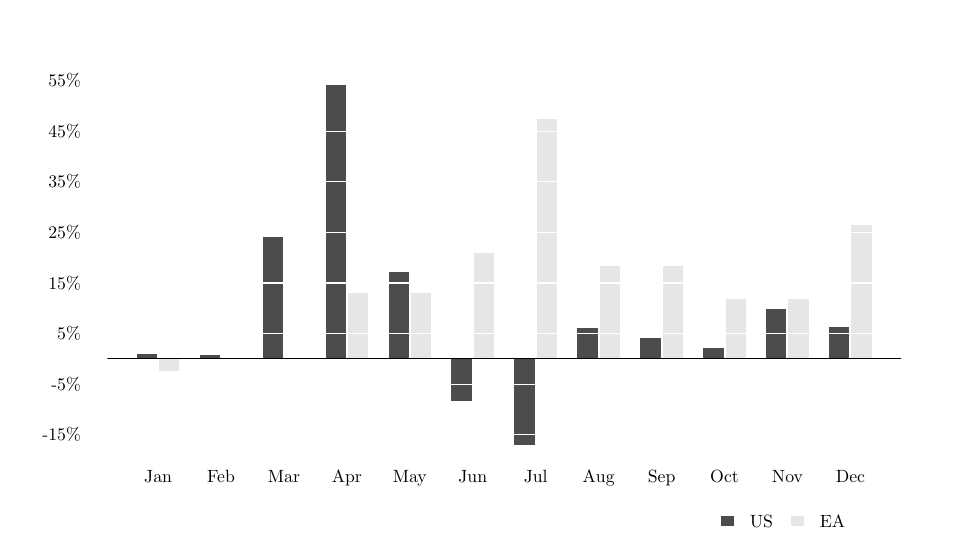
\begin{tikzpicture}[x=1pt,y=1pt]
\definecolor{fillColor}{RGB}{255,255,255}
\path[use as bounding box,fill=fillColor,fill opacity=0.00] (0,0) rectangle (325.21,180.67);
\begin{scope}
\path[clip] (  0.00,  0.00) rectangle (325.21,180.67);
\definecolor{fillColor}{gray}{0.30}

\path[fill=fillColor] ( 39.42, 61.00) rectangle ( 46.76, 62.66);
\definecolor{fillColor}{RGB}{230,230,230}

\path[fill=fillColor] ( 47.49, 61.00) rectangle ( 54.83, 56.73);
\definecolor{fillColor}{gray}{0.30}

\path[fill=fillColor] ( 62.16, 61.00) rectangle ( 69.50, 62.23);
\definecolor{fillColor}{RGB}{230,230,230}

\path[fill=fillColor] ( 70.23, 61.00) rectangle ( 77.57, 61.34);
\definecolor{fillColor}{gray}{0.30}

\path[fill=fillColor] ( 84.91, 61.00) rectangle ( 92.24,105.06);
\definecolor{fillColor}{RGB}{230,230,230}

\path[fill=fillColor] ( 92.98, 61.00) rectangle (100.31, 61.34);
\definecolor{fillColor}{gray}{0.30}

\path[fill=fillColor] (107.65, 61.00) rectangle (114.99,159.88);
\definecolor{fillColor}{RGB}{230,230,230}

\path[fill=fillColor] (115.72, 61.00) rectangle (123.06, 84.87);
\definecolor{fillColor}{gray}{0.30}

\path[fill=fillColor] (130.39, 61.00) rectangle (137.73, 92.31);
\definecolor{fillColor}{RGB}{230,230,230}

\path[fill=fillColor] (138.46, 61.00) rectangle (145.80, 84.87);
\definecolor{fillColor}{gray}{0.30}

\path[fill=fillColor] (153.13, 61.00) rectangle (160.47, 45.83);
\definecolor{fillColor}{RGB}{230,230,230}

\path[fill=fillColor] (161.20, 61.00) rectangle (168.54, 99.34);
\definecolor{fillColor}{gray}{0.30}

\path[fill=fillColor] (175.88, 61.00) rectangle (183.21, 30.01);
\definecolor{fillColor}{RGB}{230,230,230}

\path[fill=fillColor] (183.95, 61.00) rectangle (191.28,147.63);
\definecolor{fillColor}{gray}{0.30}

\path[fill=fillColor] (198.62, 61.00) rectangle (205.95, 72.01);
\definecolor{fillColor}{RGB}{230,230,230}

\path[fill=fillColor] (206.69, 61.00) rectangle (214.02, 94.70);
\definecolor{fillColor}{gray}{0.30}

\path[fill=fillColor] (221.36, 61.00) rectangle (228.70, 68.50);
\definecolor{fillColor}{RGB}{230,230,230}

\path[fill=fillColor] (229.43, 61.00) rectangle (236.77, 94.70);
\definecolor{fillColor}{gray}{0.30}

\path[fill=fillColor] (244.10, 61.00) rectangle (251.44, 64.79);
\definecolor{fillColor}{RGB}{230,230,230}

\path[fill=fillColor] (252.17, 61.00) rectangle (259.51, 82.67);
\definecolor{fillColor}{gray}{0.30}

\path[fill=fillColor] (266.84, 61.00) rectangle (274.18, 79.09);
\definecolor{fillColor}{RGB}{230,230,230}

\path[fill=fillColor] (274.91, 61.00) rectangle (282.25, 82.67);
\definecolor{fillColor}{gray}{0.30}

\path[fill=fillColor] (289.59, 61.00) rectangle (296.92, 72.67);
\definecolor{fillColor}{RGB}{230,230,230}

\path[fill=fillColor] (297.66, 61.00) rectangle (304.99,109.42);
\end{scope}
\begin{scope}
\path[clip] (  0.00,  0.00) rectangle (325.21,180.67);
\definecolor{drawColor}{RGB}{0,0,0}

\node[text=drawColor,anchor=base,inner sep=0pt, outer sep=0pt, scale=  0.64] at ( 47.13, 16.32) {Jan};

\node[text=drawColor,anchor=base,inner sep=0pt, outer sep=0pt, scale=  0.64] at ( 69.87, 16.32) {Feb};

\node[text=drawColor,anchor=base,inner sep=0pt, outer sep=0pt, scale=  0.64] at ( 92.61, 16.32) {Mar};

\node[text=drawColor,anchor=base,inner sep=0pt, outer sep=0pt, scale=  0.64] at (115.35, 16.32) {Apr};

\node[text=drawColor,anchor=base,inner sep=0pt, outer sep=0pt, scale=  0.64] at (138.09, 16.32) {May};

\node[text=drawColor,anchor=base,inner sep=0pt, outer sep=0pt, scale=  0.64] at (160.84, 16.32) {Jun};

\node[text=drawColor,anchor=base,inner sep=0pt, outer sep=0pt, scale=  0.64] at (183.58, 16.32) {Jul};

\node[text=drawColor,anchor=base,inner sep=0pt, outer sep=0pt, scale=  0.64] at (206.32, 16.32) {Aug};

\node[text=drawColor,anchor=base,inner sep=0pt, outer sep=0pt, scale=  0.64] at (229.06, 16.32) {Sep};

\node[text=drawColor,anchor=base,inner sep=0pt, outer sep=0pt, scale=  0.64] at (251.80, 16.32) {Oct};

\node[text=drawColor,anchor=base,inner sep=0pt, outer sep=0pt, scale=  0.64] at (274.55, 16.32) {Nov};

\node[text=drawColor,anchor=base,inner sep=0pt, outer sep=0pt, scale=  0.64] at (297.29, 16.32) {Dec};
\end{scope}
\begin{scope}
\path[clip] ( 28.80, 33.60) rectangle (315.62,161.47);
\definecolor{drawColor}{RGB}{0,0,0}

\path[draw=drawColor,line width= 0.4pt,line join=round,line cap=round] ( 28.80, 61.00) -- (315.62, 61.00);
\end{scope}
\begin{scope}
\path[clip] (  0.00,  0.00) rectangle (325.21,180.67);
\definecolor{drawColor}{RGB}{0,0,0}

\node[text=drawColor,anchor=base east,inner sep=0pt, outer sep=0pt, scale=  0.64] at ( 19.20, 31.40) {-15\%};

\node[text=drawColor,anchor=base east,inner sep=0pt, outer sep=0pt, scale=  0.64] at ( 19.20, 49.66) {-5\%};

\node[text=drawColor,anchor=base east,inner sep=0pt, outer sep=0pt, scale=  0.64] at ( 19.20, 67.93) {5\%};

\node[text=drawColor,anchor=base east,inner sep=0pt, outer sep=0pt, scale=  0.64] at ( 19.20, 86.20) {15\%};

\node[text=drawColor,anchor=base east,inner sep=0pt, outer sep=0pt, scale=  0.64] at ( 19.20,104.47) {25\%};

\node[text=drawColor,anchor=base east,inner sep=0pt, outer sep=0pt, scale=  0.64] at ( 19.20,122.74) {35\%};

\node[text=drawColor,anchor=base east,inner sep=0pt, outer sep=0pt, scale=  0.64] at ( 19.20,141.00) {45\%};

\node[text=drawColor,anchor=base east,inner sep=0pt, outer sep=0pt, scale=  0.64] at ( 19.20,159.27) {55\%};
\end{scope}
\begin{scope}
\path[clip] ( 28.80, 33.60) rectangle (315.62,161.47);
\definecolor{drawColor}{RGB}{255,255,255}

\path[draw=drawColor,line width= 0.4pt,line join=round,line cap=round] ( 28.80, 33.60) -- (315.62, 33.60);

\path[draw=drawColor,line width= 0.4pt,line join=round,line cap=round] ( 28.80, 51.87) -- (315.62, 51.87);

\path[draw=drawColor,line width= 0.4pt,line join=round,line cap=round] ( 28.80, 70.14) -- (315.62, 70.14);

\path[draw=drawColor,line width= 0.4pt,line join=round,line cap=round] ( 28.80, 88.40) -- (315.62, 88.40);

\path[draw=drawColor,line width= 0.4pt,line join=round,line cap=round] ( 28.80,106.67) -- (315.62,106.67);

\path[draw=drawColor,line width= 0.4pt,line join=round,line cap=round] ( 28.80,124.94) -- (315.62,124.94);

\path[draw=drawColor,line width= 0.4pt,line join=round,line cap=round] ( 28.80,143.21) -- (315.62,143.21);

\path[draw=drawColor,line width= 0.4pt,line join=round,line cap=round] ( 28.80,161.47) -- (315.62,161.47);
\end{scope}
\begin{scope}
\path[clip] (  0.00,  0.00) rectangle (325.21,180.67);
\definecolor{fillColor}{gray}{0.30}

\path[fill=fillColor, yshift = -12.5] (250.60, 16.88) rectangle (255.20, 13.04);
\definecolor{fillColor}{RGB}{230,230,230}

\path[fill=fillColor, yshift = -12.5] (275.88, 16.88) rectangle (280.48, 13.04);
\definecolor{drawColor}{RGB}{0,0,0}

\node[text=drawColor,anchor=base west,inner sep=0pt, outer sep=0pt, scale=  0.64, yshift = -20] at (260.96, 12.76) {US};

\node[text=drawColor,anchor=base west,inner sep=0pt, outer sep=0pt, scale=  0.64, yshift = -20] at (286.24, 12.76) {EA};
\end{scope}
\end{tikzpicture}

\end{figure} 
	
\end{frame}


\section{Macroeconomic Outcomes}

\begin{frame}{Industrial Production Post GFC and COVID-19 Pandemic}

\begin{figure}[h!]
     \centering
     % Created by tikzDevice version 0.12.5 on 2023-11-24 23:42:35
% !TEX encoding = UTF-8 Unicode
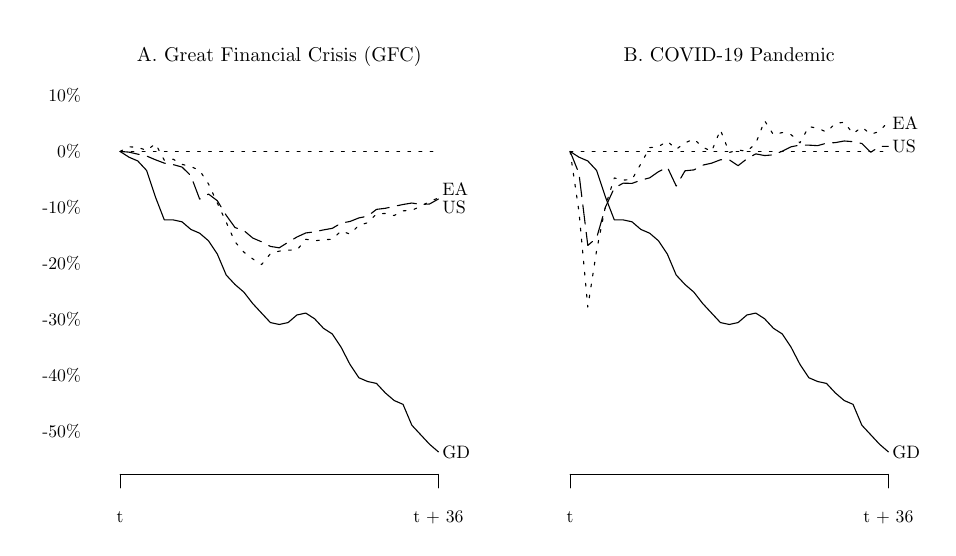
\begin{tikzpicture}[x=1pt,y=1pt]
\definecolor{fillColor}{RGB}{255,255,255}
\path[use as bounding box,fill=fillColor,fill opacity=0.00] (0,0) rectangle (325.21,180.67);
\begin{scope}
\path[clip] ( 28.80, 19.20) rectangle (153.01,161.47);
\definecolor{drawColor}{RGB}{0,0,0}

\path[draw=drawColor,line width= 0.4pt,line join=round,line cap=round] ( 33.40,135.94) --
	( 36.59,133.88) --
	( 39.79,132.50) --
	( 42.98,129.07) --
	( 46.18,119.45) --
	( 49.37,111.21) --
	( 52.57,111.21) --
	( 55.76,110.52) --
	( 58.96,107.77) --
	( 62.15,106.40) --
	( 65.35,103.65) --
	( 68.54, 98.84) --
	( 71.74, 91.28) --
	( 74.93, 87.85) --
	( 78.13, 85.10) --
	( 81.32, 80.98) --
	( 84.51, 77.54) --
	( 87.71, 74.11) --
	( 90.90, 73.42) --
	( 94.10, 74.11) --
	( 97.29, 76.85) --
	(100.49, 77.54) --
	(103.68, 75.48) --
	(106.88, 72.04) --
	(110.07, 69.99) --
	(113.27, 65.17) --
	(116.46, 58.99) --
	(119.66, 54.18) --
	(122.85, 52.81) --
	(126.04, 52.12) --
	(129.24, 48.69) --
	(132.43, 45.94) --
	(135.63, 44.56) --
	(138.82, 37.01) --
	(142.02, 33.57) --
	(145.21, 30.14) --
	(148.41, 27.39);
\end{scope}
\begin{scope}
\path[clip] ( 28.80, 19.20) rectangle (153.01,161.47);
\definecolor{drawColor}{RGB}{0,0,0}

\path[draw=drawColor,line width= 0.4pt,dash pattern=on 1pt off 3pt ,line join=round,line cap=round] ( 33.40,135.94) --
	(148.41,135.94);
\end{scope}
\begin{scope}
\path[clip] (  0.00,  0.00) rectangle (325.21,180.67);
\definecolor{drawColor}{RGB}{0,0,0}

\path[draw=drawColor,line width= 0.4pt,line join=round,line cap=round] ( 33.40, 19.20) -- (148.41, 19.20);

\path[draw=drawColor,line width= 0.4pt,line join=round,line cap=round] ( 33.40, 19.20) -- ( 33.40, 14.40);

\path[draw=drawColor,line width= 0.4pt,line join=round,line cap=round] (148.41, 19.20) -- (148.41, 14.40);

\node[text=drawColor,anchor=base,inner sep=0pt, outer sep=0pt, scale=  0.64] at ( 33.40,  1.92) {t};

\node[text=drawColor,anchor=base,inner sep=0pt, outer sep=0pt, scale=  0.64] at (148.41,  1.92) {t + 36};

\node[text=drawColor,anchor=base east,inner sep=0pt, outer sep=0pt, scale=  0.64] at ( 19.20, 32.40) {-50\%};

\node[text=drawColor,anchor=base east,inner sep=0pt, outer sep=0pt, scale=  0.64] at ( 19.20, 52.67) {-40\%};

\node[text=drawColor,anchor=base east,inner sep=0pt, outer sep=0pt, scale=  0.64] at ( 19.20, 72.93) {-30\%};

\node[text=drawColor,anchor=base east,inner sep=0pt, outer sep=0pt, scale=  0.64] at ( 19.20, 93.20) {-20\%};

\node[text=drawColor,anchor=base east,inner sep=0pt, outer sep=0pt, scale=  0.64] at ( 19.20,113.47) {-10\%};

\node[text=drawColor,anchor=base east,inner sep=0pt, outer sep=0pt, scale=  0.64] at ( 19.20,133.73) {0\%};

\node[text=drawColor,anchor=base east,inner sep=0pt, outer sep=0pt, scale=  0.64] at ( 19.20,154.00) {10\%};

\node[text=drawColor,anchor=base west,inner sep=0pt, outer sep=0pt, scale=  0.65] at (149.84, 25.15) {GD};
\end{scope}
\begin{scope}
\path[clip] ( 28.80, 19.20) rectangle (153.01,161.47);
\definecolor{drawColor}{RGB}{0,0,0}

\path[draw=drawColor,line width= 0.4pt,dash pattern=on 7pt off 3pt ,line join=round,line cap=round] ( 33.40,135.94) --
	( 36.59,135.70) --
	( 39.79,134.96) --
	( 42.98,134.30) --
	( 46.18,132.93) --
	( 49.37,131.72) --
	( 52.57,131.19) --
	( 55.76,130.31) --
	( 58.96,127.19) --
	( 62.15,118.69) --
	( 65.35,120.55) --
	( 68.54,118.12) --
	( 71.74,112.88) --
	( 74.93,108.43) --
	( 78.13,107.36) --
	( 81.32,104.66) --
	( 84.51,103.29) --
	( 87.71,101.63) --
	( 90.90,101.12) --
	( 94.10,103.13) --
	( 97.29,105.02) --
	(100.49,106.49) --
	(103.68,106.89) --
	(106.88,107.59) --
	(110.07,108.16) --
	(113.27,110.04) --
	(116.46,110.64) --
	(119.66,111.92) --
	(122.85,112.55) --
	(126.04,115.01) --
	(129.24,115.40) --
	(132.43,116.10) --
	(135.63,116.77) --
	(138.82,117.30) --
	(142.02,116.80) --
	(145.21,116.95) --
	(148.41,118.74);
\end{scope}
\begin{scope}
\path[clip] (  0.00,  0.00) rectangle (325.21,180.67);
\definecolor{drawColor}{RGB}{0,0,0}

\node[text=drawColor,anchor=base west,inner sep=0pt, outer sep=0pt, scale=  0.65] at (149.84,113.43) {US};
\end{scope}
\begin{scope}
\path[clip] ( 28.80, 19.20) rectangle (153.01,161.47);
\definecolor{drawColor}{RGB}{0,0,0}

\path[draw=drawColor,line width= 0.4pt,dash pattern=on 1pt off 3pt ,line join=round,line cap=round] ( 33.40,135.94) --
	( 36.59,137.62) --
	( 39.79,137.43) --
	( 42.98,136.31) --
	( 46.18,138.74) --
	( 49.37,132.77) --
	( 52.57,133.14) --
	( 55.76,131.27) --
	( 58.96,130.53) --
	( 62.15,129.03) --
	( 65.35,124.18) --
	( 68.54,117.28) --
	( 71.74,110.37) --
	( 74.93,103.28) --
	( 78.13, 99.55) --
	( 81.32, 97.12) --
	( 84.51, 95.07) --
	( 87.71, 98.99) --
	( 90.90, 99.92) --
	( 94.10,100.29) --
	( 97.29,100.29) --
	(100.49,104.21) --
	(103.68,103.65) --
	(106.88,104.03) --
	(110.07,104.21) --
	(113.27,107.20) --
	(116.46,106.08) --
	(119.66,109.25) --
	(122.85,110.18) --
	(126.04,113.36) --
	(129.24,113.54) --
	(132.43,112.80) --
	(135.63,114.48) --
	(138.82,114.66) --
	(142.02,116.16) --
	(145.21,117.84) --
	(148.41,119.14);
\end{scope}
\begin{scope}
\path[clip] (  0.00,  0.00) rectangle (325.21,180.67);
\definecolor{drawColor}{RGB}{0,0,0}

\node[text=drawColor,anchor=base west,inner sep=0pt, outer sep=0pt, scale=  0.65] at (149.84,119.92) {EA};
\end{scope}
\begin{scope}
\path[clip] (  0.00,  0.00) rectangle (162.61,180.67);
\definecolor{drawColor}{RGB}{0,0,0}

\node[text=drawColor,anchor=base,inner sep=0pt, outer sep=0pt, scale=  0.72] at ( 90.90,168.60) {A. Great Financial Crisis (GFC)};
\end{scope}
\begin{scope}
\path[clip] (191.41, 19.20) rectangle (315.62,161.47);
\definecolor{drawColor}{RGB}{0,0,0}

\path[draw=drawColor,line width= 0.4pt,line join=round,line cap=round] (196.01,135.94) --
	(199.20,133.88) --
	(202.40,132.50) --
	(205.59,129.07) --
	(208.79,119.45) --
	(211.98,111.21) --
	(215.18,111.21) --
	(218.37,110.52) --
	(221.56,107.77) --
	(224.76,106.40) --
	(227.95,103.65) --
	(231.15, 98.84) --
	(234.34, 91.28) --
	(237.54, 87.85) --
	(240.73, 85.10) --
	(243.93, 80.98) --
	(247.12, 77.54) --
	(250.32, 74.11) --
	(253.51, 73.42) --
	(256.71, 74.11) --
	(259.90, 76.85) --
	(263.10, 77.54) --
	(266.29, 75.48) --
	(269.48, 72.04) --
	(272.68, 69.99) --
	(275.87, 65.17) --
	(279.07, 58.99) --
	(282.26, 54.18) --
	(285.46, 52.81) --
	(288.65, 52.12) --
	(291.85, 48.69) --
	(295.04, 45.94) --
	(298.24, 44.56) --
	(301.43, 37.01) --
	(304.63, 33.57) --
	(307.82, 30.14) --
	(311.01, 27.39);
\end{scope}
\begin{scope}
\path[clip] (191.41, 19.20) rectangle (315.62,161.47);
\definecolor{drawColor}{RGB}{0,0,0}

\path[draw=drawColor,line width= 0.4pt,dash pattern=on 1pt off 3pt ,line join=round,line cap=round] (196.01,135.94) --
	(311.01,135.94);
\end{scope}
\begin{scope}
\path[clip] (  0.00,  0.00) rectangle (325.21,180.67);
\definecolor{drawColor}{RGB}{0,0,0}

\path[draw=drawColor,line width= 0.4pt,line join=round,line cap=round] (196.01, 19.20) -- (311.01, 19.20);

\path[draw=drawColor,line width= 0.4pt,line join=round,line cap=round] (196.01, 19.20) -- (196.01, 14.40);

\path[draw=drawColor,line width= 0.4pt,line join=round,line cap=round] (311.01, 19.20) -- (311.01, 14.40);

\node[text=drawColor,anchor=base,inner sep=0pt, outer sep=0pt, scale=  0.64] at (196.01,  1.92) {t};

\node[text=drawColor,anchor=base,inner sep=0pt, outer sep=0pt, scale=  0.64] at (311.01,  1.92) {t + 36};

\node[text=drawColor,anchor=base west,inner sep=0pt, outer sep=0pt, scale=  0.65] at (312.45, 25.15) {GD};
\end{scope}
\begin{scope}
\path[clip] (191.41, 19.20) rectangle (315.62,161.47);
\definecolor{drawColor}{RGB}{0,0,0}

\path[draw=drawColor,line width= 0.4pt,dash pattern=on 7pt off 3pt ,line join=round,line cap=round] (196.01,135.94) --
	(199.20,128.03) --
	(202.40,101.97) --
	(205.59,104.71) --
	(208.79,115.86) --
	(211.98,122.74) --
	(215.18,124.48) --
	(218.37,124.40) --
	(221.56,125.56) --
	(224.76,126.41) --
	(227.95,128.64) --
	(231.15,130.26) --
	(234.34,123.46) --
	(237.54,128.96) --
	(240.73,129.27) --
	(243.93,130.99) --
	(247.12,131.70) --
	(250.32,132.93) --
	(253.51,132.93) --
	(256.71,130.81) --
	(259.90,133.29) --
	(263.10,135.07) --
	(266.29,134.45) --
	(269.48,134.72) --
	(272.68,136.03) --
	(275.87,137.62) --
	(279.07,138.26) --
	(282.26,138.22) --
	(285.46,138.04) --
	(288.65,138.93) --
	(291.85,139.13) --
	(295.04,139.72) --
	(298.24,139.48) --
	(301.43,138.81) --
	(304.63,135.64) --
	(307.82,137.76) --
	(311.01,137.80);
\end{scope}
\begin{scope}
\path[clip] (  0.00,  0.00) rectangle (325.21,180.67);
\definecolor{drawColor}{RGB}{0,0,0}

\node[text=drawColor,anchor=base west,inner sep=0pt, outer sep=0pt, scale=  0.65] at (312.45,135.73) {US};
\end{scope}
\begin{scope}
\path[clip] (191.41, 19.20) rectangle (315.62,161.47);
\definecolor{drawColor}{RGB}{0,0,0}

\path[draw=drawColor,line width= 0.4pt,dash pattern=on 1pt off 3pt ,line join=round,line cap=round] (196.01,135.94) --
	(199.20,114.27) --
	(202.40, 79.71) --
	(205.59,100.21) --
	(208.79,116.22) --
	(211.98,126.37) --
	(215.18,125.59) --
	(218.37,125.79) --
	(221.56,131.45) --
	(224.76,137.31) --
	(227.95,137.70) --
	(231.15,139.65) --
	(234.34,136.72) --
	(237.54,139.06) --
	(240.73,140.43) --
	(243.93,137.50) --
	(247.12,135.94) --
	(250.32,143.75) --
	(253.51,135.55) --
	(256.71,136.52) --
	(259.90,135.94) --
	(263.10,138.87) --
	(266.29,147.07) --
	(269.48,141.99) --
	(272.68,142.77) --
	(275.87,141.99) --
	(279.07,139.06) --
	(282.26,144.92) --
	(285.46,144.33) --
	(288.65,142.97) --
	(291.85,146.09) --
	(295.04,146.48) --
	(298.24,142.38) --
	(301.43,144.72) --
	(304.63,142.19) --
	(307.82,143.16) --
	(311.01,146.87);
\end{scope}
\begin{scope}
\path[clip] (  0.00,  0.00) rectangle (325.21,180.67);
\definecolor{drawColor}{RGB}{0,0,0}

\node[text=drawColor,anchor=base west,inner sep=0pt, outer sep=0pt, scale=  0.65] at (312.45,143.83) {EA};
\end{scope}
\begin{scope}
\path[clip] (162.61,  0.00) rectangle (325.21,180.67);
\definecolor{drawColor}{RGB}{0,0,0}

\node[text=drawColor,anchor=base,inner sep=0pt, outer sep=0pt, scale=  0.72] at (253.51,168.60) {B. COVID-19 Pandemic};
\end{scope}
\end{tikzpicture}

\end{figure} 
	
\end{frame}

\begin{frame}{Employment Post GFC and COVID-19 Pandemic}

\begin{figure}[h!]
     \centering
     % Created by tikzDevice version 0.12.5 on 2023-11-24 23:42:35
% !TEX encoding = UTF-8 Unicode
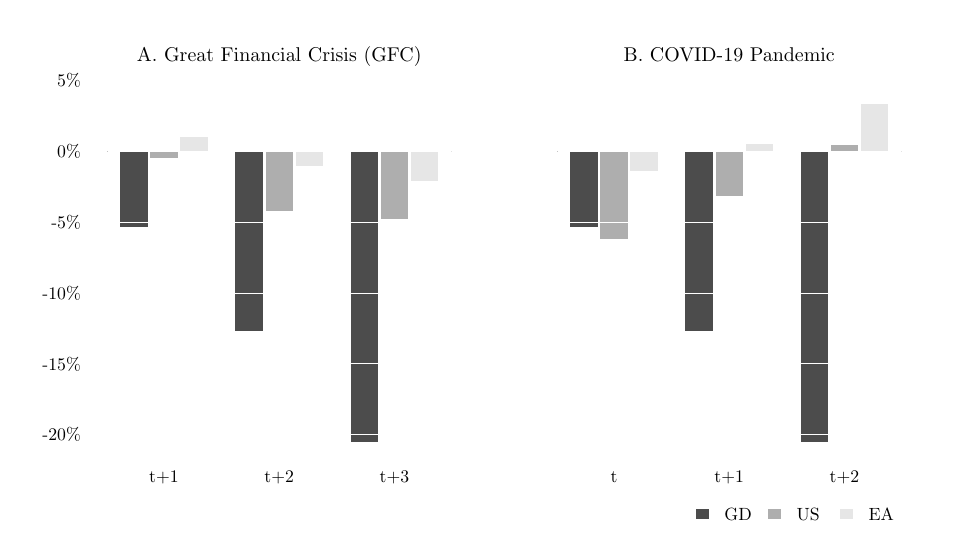
\begin{tikzpicture}[x=1pt,y=1pt]
\definecolor{fillColor}{RGB}{255,255,255}
\path[use as bounding box,fill=fillColor,fill opacity=0.00] (0,0) rectangle (325.21,180.67);
\begin{scope}
\path[clip] (  0.00,  0.00) rectangle (162.61,180.67);
\definecolor{fillColor}{gray}{0.30}

\path[fill=fillColor] ( 33.40,135.90) rectangle ( 43.31,108.47);
\definecolor{fillColor}{RGB}{174,174,174}

\path[fill=fillColor] ( 44.31,135.90) rectangle ( 54.22,133.50);
\definecolor{fillColor}{RGB}{230,230,230}

\path[fill=fillColor] ( 55.21,135.90) rectangle ( 65.13,141.05);
\definecolor{fillColor}{gray}{0.30}

\path[fill=fillColor] ( 75.04,135.90) rectangle ( 84.96, 70.99);
\definecolor{fillColor}{RGB}{174,174,174}

\path[fill=fillColor] ( 85.95,135.90) rectangle ( 95.86,114.29);
\definecolor{fillColor}{RGB}{230,230,230}

\path[fill=fillColor] ( 96.85,135.90) rectangle (106.77,130.64);
\definecolor{fillColor}{gray}{0.30}

\path[fill=fillColor] (116.68,135.90) rectangle (126.60, 30.87);
\definecolor{fillColor}{RGB}{174,174,174}

\path[fill=fillColor] (127.59,135.90) rectangle (137.50,111.44);
\definecolor{fillColor}{RGB}{230,230,230}

\path[fill=fillColor] (138.49,135.90) rectangle (148.41,125.35);
\end{scope}
\begin{scope}
\path[clip] (  0.00,  0.00) rectangle (325.21,180.67);
\definecolor{drawColor}{RGB}{0,0,0}

\node[text=drawColor,anchor=base,inner sep=0pt, outer sep=0pt, scale=  0.64] at ( 49.26, 16.32) {t+1};

\node[text=drawColor,anchor=base,inner sep=0pt, outer sep=0pt, scale=  0.64] at ( 90.90, 16.32) {t+2};

\node[text=drawColor,anchor=base,inner sep=0pt, outer sep=0pt, scale=  0.64] at (132.54, 16.32) {t+3};
\end{scope}
\begin{scope}
\path[clip] ( 28.80, 33.60) rectangle (153.01,161.47);
\definecolor{drawColor}{RGB}{0,0,0}

\path[draw=drawColor,line width= 0.4pt,line join=round,line cap=round] ( 28.80,135.90) -- (153.01,135.90);
\end{scope}
\begin{scope}
\path[clip] (  0.00,  0.00) rectangle (325.21,180.67);
\definecolor{drawColor}{RGB}{0,0,0}

\node[text=drawColor,anchor=base east,inner sep=0pt, outer sep=0pt, scale=  0.64] at ( 19.20, 31.40) {-20\%};

\node[text=drawColor,anchor=base east,inner sep=0pt, outer sep=0pt, scale=  0.64] at ( 19.20, 56.97) {-15\%};

\node[text=drawColor,anchor=base east,inner sep=0pt, outer sep=0pt, scale=  0.64] at ( 19.20, 82.55) {-10\%};

\node[text=drawColor,anchor=base east,inner sep=0pt, outer sep=0pt, scale=  0.64] at ( 19.20,108.12) {-5\%};

\node[text=drawColor,anchor=base east,inner sep=0pt, outer sep=0pt, scale=  0.64] at ( 19.20,133.70) {0\%};

\node[text=drawColor,anchor=base east,inner sep=0pt, outer sep=0pt, scale=  0.64] at ( 19.20,159.27) {5\%};
\end{scope}
\begin{scope}
\path[clip] ( 28.80, 33.60) rectangle (153.01,161.47);
\definecolor{drawColor}{RGB}{255,255,255}

\path[draw=drawColor,line width= 0.4pt,line join=round,line cap=round] ( 28.80, 33.60) -- (153.01, 33.60);

\path[draw=drawColor,line width= 0.4pt,line join=round,line cap=round] ( 28.80, 59.17) -- (153.01, 59.17);

\path[draw=drawColor,line width= 0.4pt,line join=round,line cap=round] ( 28.80, 84.75) -- (153.01, 84.75);

\path[draw=drawColor,line width= 0.4pt,line join=round,line cap=round] ( 28.80,110.33) -- (153.01,110.33);

\path[draw=drawColor,line width= 0.4pt,line join=round,line cap=round] ( 28.80,135.90) -- (153.01,135.90);

\path[draw=drawColor,line width= 0.4pt,line join=round,line cap=round] ( 28.80,161.47) -- (153.01,161.47);
\end{scope}
\begin{scope}
\path[clip] (  0.00,  0.00) rectangle (162.61,180.67);
\definecolor{drawColor}{RGB}{0,0,0}

\node[text=drawColor,anchor=base,inner sep=0pt, outer sep=0pt, scale=  0.72] at ( 90.90,168.60) {A. Great Financial Crisis (GFC)};
\end{scope}
\begin{scope}
\path[clip] (162.61,  0.00) rectangle (325.21,180.67);
\definecolor{fillColor}{gray}{0.30}

\path[fill=fillColor] (196.01,135.90) rectangle (205.92,108.47);
\definecolor{fillColor}{RGB}{174,174,174}

\path[fill=fillColor] (206.91,135.90) rectangle (216.83,104.27);
\definecolor{fillColor}{RGB}{230,230,230}

\path[fill=fillColor] (217.82,135.90) rectangle (227.73,128.84);
\definecolor{fillColor}{gray}{0.30}

\path[fill=fillColor] (237.65,135.90) rectangle (247.56, 70.99);
\definecolor{fillColor}{RGB}{174,174,174}

\path[fill=fillColor] (248.55,135.90) rectangle (258.47,119.80);
\definecolor{fillColor}{RGB}{230,230,230}

\path[fill=fillColor] (259.46,135.90) rectangle (269.37,138.54);
\definecolor{fillColor}{gray}{0.30}

\path[fill=fillColor] (279.29,135.90) rectangle (289.20, 30.87);
\definecolor{fillColor}{RGB}{174,174,174}

\path[fill=fillColor] (290.19,135.90) rectangle (300.11,138.34);
\definecolor{fillColor}{RGB}{230,230,230}

\path[fill=fillColor] (301.10,135.90) rectangle (311.01,152.93);
\end{scope}
\begin{scope}
\path[clip] (  0.00,  0.00) rectangle (325.21,180.67);
\definecolor{drawColor}{RGB}{0,0,0}

\node[text=drawColor,anchor=base,inner sep=0pt, outer sep=0pt, scale=  0.64] at (211.87, 16.32) {t};

\node[text=drawColor,anchor=base,inner sep=0pt, outer sep=0pt, scale=  0.64] at (253.51, 16.32) {t+1};

\node[text=drawColor,anchor=base,inner sep=0pt, outer sep=0pt, scale=  0.64] at (295.15, 16.32) {t+2};
\end{scope}
\begin{scope}
\path[clip] (191.41, 33.60) rectangle (315.62,161.47);
\definecolor{drawColor}{RGB}{0,0,0}

\path[draw=drawColor,line width= 0.4pt,line join=round,line cap=round] (191.41,135.90) -- (315.62,135.90);
\definecolor{drawColor}{RGB}{255,255,255}

\path[draw=drawColor,line width= 0.4pt,line join=round,line cap=round] (191.41, 33.60) -- (315.62, 33.60);

\path[draw=drawColor,line width= 0.4pt,line join=round,line cap=round] (191.41, 59.17) -- (315.62, 59.17);

\path[draw=drawColor,line width= 0.4pt,line join=round,line cap=round] (191.41, 84.75) -- (315.62, 84.75);

\path[draw=drawColor,line width= 0.4pt,line join=round,line cap=round] (191.41,110.33) -- (315.62,110.33);

\path[draw=drawColor,line width= 0.4pt,line join=round,line cap=round] (191.41,135.90) -- (315.62,135.90);

\path[draw=drawColor,line width= 0.4pt,line join=round,line cap=round] (191.41,161.47) -- (315.62,161.47);
\end{scope}
\begin{scope}
\path[clip] (162.61,  0.00) rectangle (325.21,180.67);
\definecolor{fillColor}{gray}{0.30}

\path[fill=fillColor] (241.43,  6.87) rectangle (246.03,  3.03);
\definecolor{fillColor}{RGB}{174,174,174}

\path[fill=fillColor] (267.46,  6.87) rectangle (272.07,  3.03);
\definecolor{fillColor}{RGB}{230,230,230}

\path[fill=fillColor] (293.50,  6.87) rectangle (298.11,  3.03);
\definecolor{drawColor}{RGB}{0,0,0}

\node[text=drawColor,anchor=base west,inner sep=0pt, outer sep=0pt, scale=  0.64] at (251.79,  2.74) {GD};

\node[text=drawColor,anchor=base west,inner sep=0pt, outer sep=0pt, scale=  0.64] at (277.83,  2.74) {US};

\node[text=drawColor,anchor=base west,inner sep=0pt, outer sep=0pt, scale=  0.64] at (303.87,  2.74) {EA};

\node[text=drawColor,anchor=base,inner sep=0pt, outer sep=0pt, scale=  0.72] at (253.51,168.60) {B. COVID-19 Pandemic};
\end{scope}
\end{tikzpicture}

\end{figure} 
	
\end{frame}

\begin{frame}{Stock Markets Post GFC and COVID-19 Pandemic}

\begin{figure}[h!]
     \centering
     % Created by tikzDevice version 0.12.5 on 2023-11-24 23:42:35
% !TEX encoding = UTF-8 Unicode
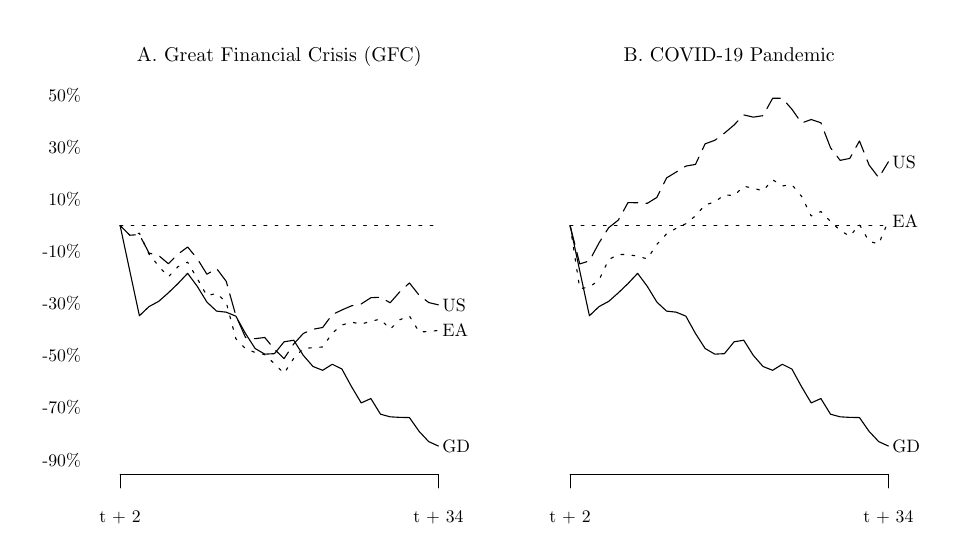
\begin{tikzpicture}[x=1pt,y=1pt]
\definecolor{fillColor}{RGB}{255,255,255}
\path[use as bounding box,fill=fillColor,fill opacity=0.00] (0,0) rectangle (325.21,180.67);
\begin{scope}
\path[clip] ( 28.80, 19.20) rectangle (153.01,161.47);
\definecolor{drawColor}{RGB}{0,0,0}

\path[draw=drawColor,line width= 0.4pt,line join=round,line cap=round] ( 33.40,109.16) --
	( 36.89, 92.80) --
	( 40.37, 76.57) --
	( 43.86, 79.89) --
	( 47.34, 81.77) --
	( 50.83, 84.85) --
	( 54.31, 88.20) --
	( 57.80, 91.91) --
	( 61.28, 87.20) --
	( 64.77, 81.50) --
	( 68.25, 78.25) --
	( 71.74, 77.87) --
	( 75.22, 76.43) --
	( 78.71, 70.16) --
	( 82.19, 64.73) --
	( 85.68, 62.70) --
	( 89.16, 62.87) --
	( 92.65, 67.15) --
	( 96.13, 67.74) --
	( 99.62, 62.23) --
	(103.10, 58.24) --
	(106.59, 56.86) --
	(110.07, 59.04) --
	(113.56, 57.30) --
	(117.04, 50.91) --
	(120.53, 45.07) --
	(124.01, 46.66) --
	(127.50, 41.00) --
	(130.98, 40.05) --
	(134.47, 39.85) --
	(137.95, 39.78) --
	(141.44, 34.80) --
	(144.92, 31.08) --
	(148.41, 29.50);
\end{scope}
\begin{scope}
\path[clip] ( 28.80, 19.20) rectangle (153.01,161.47);
\definecolor{drawColor}{RGB}{0,0,0}

\path[draw=drawColor,line width= 0.4pt,dash pattern=on 1pt off 3pt ,line join=round,line cap=round] ( 33.40,109.16) --
	(148.41,109.16);
\end{scope}
\begin{scope}
\path[clip] (  0.00,  0.00) rectangle (325.21,180.67);
\definecolor{drawColor}{RGB}{0,0,0}

\path[draw=drawColor,line width= 0.4pt,line join=round,line cap=round] ( 33.40, 19.20) -- (148.41, 19.20);

\path[draw=drawColor,line width= 0.4pt,line join=round,line cap=round] ( 33.40, 19.20) -- ( 33.40, 14.40);

\path[draw=drawColor,line width= 0.4pt,line join=round,line cap=round] (148.41, 19.20) -- (148.41, 14.40);

\node[text=drawColor,anchor=base,inner sep=0pt, outer sep=0pt, scale=  0.64] at ( 33.40,  1.92) {t + 2};

\node[text=drawColor,anchor=base,inner sep=0pt, outer sep=0pt, scale=  0.64] at (148.41,  1.92) {t + 34};

\node[text=drawColor,anchor=base east,inner sep=0pt, outer sep=0pt, scale=  0.64] at ( 19.20, 22.27) {-90\%};

\node[text=drawColor,anchor=base east,inner sep=0pt, outer sep=0pt, scale=  0.64] at ( 19.20, 41.08) {-70\%};

\node[text=drawColor,anchor=base east,inner sep=0pt, outer sep=0pt, scale=  0.64] at ( 19.20, 59.90) {-50\%};

\node[text=drawColor,anchor=base east,inner sep=0pt, outer sep=0pt, scale=  0.64] at ( 19.20, 78.72) {-30\%};

\node[text=drawColor,anchor=base east,inner sep=0pt, outer sep=0pt, scale=  0.64] at ( 19.20, 97.54) {-10\%};

\node[text=drawColor,anchor=base east,inner sep=0pt, outer sep=0pt, scale=  0.64] at ( 19.20,116.36) {10\%};

\node[text=drawColor,anchor=base east,inner sep=0pt, outer sep=0pt, scale=  0.64] at ( 19.20,135.18) {30\%};

\node[text=drawColor,anchor=base east,inner sep=0pt, outer sep=0pt, scale=  0.64] at ( 19.20,154.00) {50\%};

\node[text=drawColor,anchor=base west,inner sep=0pt, outer sep=0pt, scale=  0.65] at (149.84, 27.27) {GD};
\end{scope}
\begin{scope}
\path[clip] ( 28.80, 19.20) rectangle (153.01,161.47);
\definecolor{drawColor}{RGB}{0,0,0}

\path[draw=drawColor,line width= 0.4pt,dash pattern=on 7pt off 3pt ,line join=round,line cap=round] ( 33.40,109.16) --
	( 36.89,105.67) --
	( 40.37,105.89) --
	( 43.86, 99.22) --
	( 47.34, 98.33) --
	( 50.83, 95.38) --
	( 54.31, 98.82) --
	( 57.80,101.41) --
	( 61.28, 97.20) --
	( 64.77, 91.57) --
	( 68.25, 93.65) --
	( 71.74, 89.02) --
	( 75.22, 76.66) --
	( 78.71, 68.73) --
	( 82.19, 68.30) --
	( 85.68, 68.72) --
	( 89.16, 64.46) --
	( 92.65, 61.09) --
	( 96.13, 66.38) --
	( 99.62, 70.19) --
	(103.10, 71.69) --
	(106.59, 72.33) --
	(110.07, 77.00) --
	(113.56, 78.66) --
	(117.04, 80.17) --
	(120.53, 80.84) --
	(124.01, 83.09) --
	(127.50, 83.26) --
	(130.98, 81.26) --
	(134.47, 85.23) --
	(137.95, 88.43) --
	(141.44, 84.00) --
	(144.92, 81.35) --
	(148.41, 80.50);
\end{scope}
\begin{scope}
\path[clip] (  0.00,  0.00) rectangle (325.21,180.67);
\definecolor{drawColor}{RGB}{0,0,0}

\node[text=drawColor,anchor=base west,inner sep=0pt, outer sep=0pt, scale=  0.65] at (149.84, 78.27) {US};
\end{scope}
\begin{scope}
\path[clip] ( 28.80, 19.20) rectangle (153.01,161.47);
\definecolor{drawColor}{RGB}{0,0,0}

\path[draw=drawColor,line width= 0.4pt,dash pattern=on 1pt off 3pt ,line join=round,line cap=round] ( 33.40,109.16) --
	( 36.89,105.70) --
	( 40.37,106.38) --
	( 43.86, 98.82) --
	( 47.34, 94.51) --
	( 50.83, 90.61) --
	( 54.31, 94.29) --
	( 57.80, 95.95) --
	( 61.28, 90.01) --
	( 64.77, 83.78) --
	( 68.25, 84.70) --
	( 71.74, 81.45) --
	( 75.22, 68.28) --
	( 78.71, 64.64) --
	( 82.19, 63.31) --
	( 85.68, 62.54) --
	( 89.16, 59.21) --
	( 92.65, 55.74) --
	( 96.13, 61.17) --
	( 99.62, 64.80) --
	(103.10, 65.01) --
	(106.59, 65.30) --
	(110.07, 70.30) --
	(113.56, 73.22) --
	(117.04, 74.27) --
	(120.53, 73.54) --
	(124.01, 74.60) --
	(127.50, 75.34) --
	(130.98, 71.69) --
	(134.47, 75.13) --
	(137.95, 76.50) --
	(141.44, 70.74) --
	(144.92, 70.85) --
	(148.41, 71.27);
\end{scope}
\begin{scope}
\path[clip] (  0.00,  0.00) rectangle (325.21,180.67);
\definecolor{drawColor}{RGB}{0,0,0}

\node[text=drawColor,anchor=base west,inner sep=0pt, outer sep=0pt, scale=  0.65] at (149.84, 69.04) {EA};
\end{scope}
\begin{scope}
\path[clip] (  0.00,  0.00) rectangle (162.61,180.67);
\definecolor{drawColor}{RGB}{0,0,0}

\node[text=drawColor,anchor=base,inner sep=0pt, outer sep=0pt, scale=  0.72] at ( 90.90,168.60) {A. Great Financial Crisis (GFC)};
\end{scope}
\begin{scope}
\path[clip] (191.41, 19.20) rectangle (315.62,161.47);
\definecolor{drawColor}{RGB}{0,0,0}

\path[draw=drawColor,line width= 0.4pt,line join=round,line cap=round] (196.01,109.16) --
	(199.49, 92.80) --
	(202.98, 76.57) --
	(206.46, 79.89) --
	(209.95, 81.77) --
	(213.43, 84.85) --
	(216.92, 88.20) --
	(220.40, 91.91) --
	(223.89, 87.20) --
	(227.37, 81.50) --
	(230.86, 78.25) --
	(234.34, 77.87) --
	(237.83, 76.43) --
	(241.31, 70.16) --
	(244.80, 64.73) --
	(248.28, 62.70) --
	(251.77, 62.87) --
	(255.25, 67.15) --
	(258.74, 67.74) --
	(262.22, 62.23) --
	(265.71, 58.24) --
	(269.19, 56.86) --
	(272.68, 59.04) --
	(276.16, 57.30) --
	(279.65, 50.91) --
	(283.13, 45.07) --
	(286.62, 46.66) --
	(290.10, 41.00) --
	(293.59, 40.05) --
	(297.07, 39.85) --
	(300.56, 39.78) --
	(304.04, 34.80) --
	(307.53, 31.08) --
	(311.01, 29.50);
\end{scope}
\begin{scope}
\path[clip] (191.41, 19.20) rectangle (315.62,161.47);
\definecolor{drawColor}{RGB}{0,0,0}

\path[draw=drawColor,line width= 0.4pt,dash pattern=on 1pt off 3pt ,line join=round,line cap=round] (196.01,109.16) --
	(311.01,109.16);
\end{scope}
\begin{scope}
\path[clip] (  0.00,  0.00) rectangle (325.21,180.67);
\definecolor{drawColor}{RGB}{0,0,0}

\path[draw=drawColor,line width= 0.4pt,line join=round,line cap=round] (196.01, 19.20) -- (311.01, 19.20);

\path[draw=drawColor,line width= 0.4pt,line join=round,line cap=round] (196.01, 19.20) -- (196.01, 14.40);

\path[draw=drawColor,line width= 0.4pt,line join=round,line cap=round] (311.01, 19.20) -- (311.01, 14.40);

\node[text=drawColor,anchor=base,inner sep=0pt, outer sep=0pt, scale=  0.64] at (196.01,  1.92) {t + 2};

\node[text=drawColor,anchor=base,inner sep=0pt, outer sep=0pt, scale=  0.64] at (311.01,  1.92) {t + 34};

\node[text=drawColor,anchor=base west,inner sep=0pt, outer sep=0pt, scale=  0.65] at (312.45, 27.27) {GD};
\end{scope}
\begin{scope}
\path[clip] (191.41, 19.20) rectangle (315.62,161.47);
\definecolor{drawColor}{RGB}{0,0,0}

\path[draw=drawColor,line width= 0.4pt,dash pattern=on 7pt off 3pt ,line join=round,line cap=round] (196.01,109.16) --
	(199.49, 95.29) --
	(202.98, 96.40) --
	(206.46,102.92) --
	(209.95,108.40) --
	(213.43,111.14) --
	(216.92,117.44) --
	(220.40,117.41) --
	(223.89,117.20) --
	(227.37,119.34) --
	(230.86,126.39) --
	(234.34,128.49) --
	(237.83,130.64) --
	(241.31,131.27) --
	(244.80,138.70) --
	(248.28,139.96) --
	(251.77,142.55) --
	(255.25,145.50) --
	(258.74,149.14) --
	(262.22,148.34) --
	(265.71,148.87) --
	(269.19,155.15) --
	(272.68,155.15) --
	(276.16,151.19) --
	(279.65,146.21) --
	(283.13,147.49) --
	(286.62,146.32) --
	(290.10,137.29) --
	(293.59,132.72) --
	(297.07,133.43) --
	(300.56,139.73) --
	(304.04,131.05) --
	(307.53,126.44) --
	(311.01,132.18);
\end{scope}
\begin{scope}
\path[clip] (  0.00,  0.00) rectangle (325.21,180.67);
\definecolor{drawColor}{RGB}{0,0,0}

\node[text=drawColor,anchor=base west,inner sep=0pt, outer sep=0pt, scale=  0.65] at (312.45,129.93) {US};
\end{scope}
\begin{scope}
\path[clip] (191.41, 19.20) rectangle (315.62,161.47);
\definecolor{drawColor}{RGB}{0,0,0}

\path[draw=drawColor,line width= 0.4pt,dash pattern=on 1pt off 3pt ,line join=round,line cap=round] (196.01,109.16) --
	(199.49, 86.36) --
	(202.98, 86.90) --
	(206.46, 89.50) --
	(209.95, 96.86) --
	(213.43, 98.73) --
	(216.92, 98.69) --
	(220.40, 98.08) --
	(223.89, 97.13) --
	(227.37,102.37) --
	(230.86,106.16) --
	(234.34,108.18) --
	(237.83,109.83) --
	(241.31,112.68) --
	(244.80,116.67) --
	(248.28,117.65) --
	(251.77,120.30) --
	(255.25,119.96) --
	(258.74,123.36) --
	(262.22,122.66) --
	(265.71,121.70) --
	(269.19,125.72) --
	(272.68,123.48) --
	(276.16,123.93) --
	(279.65,119.70) --
	(283.13,112.62) --
	(286.62,114.23) --
	(290.10,110.64) --
	(293.59,107.42) --
	(297.07,105.29) --
	(300.56,109.49) --
	(304.04,103.44) --
	(307.53,102.55) --
	(311.01,110.80);
\end{scope}
\begin{scope}
\path[clip] (  0.00,  0.00) rectangle (325.21,180.67);
\definecolor{drawColor}{RGB}{0,0,0}

\node[text=drawColor,anchor=base west,inner sep=0pt, outer sep=0pt, scale=  0.65] at (312.45,108.56) {EA};
\end{scope}
\begin{scope}
\path[clip] (162.61,  0.00) rectangle (325.21,180.67);
\definecolor{drawColor}{RGB}{0,0,0}

\node[text=drawColor,anchor=base,inner sep=0pt, outer sep=0pt, scale=  0.72] at (253.51,168.60) {B. COVID-19 Pandemic};
\end{scope}
\end{tikzpicture}

\end{figure} 
	
\end{frame}

\section{Speculation in Financial Assets as a Side Effect of Policy Responses}

\begin{frame}{In Search of Higher Returns}
\begin{epigraph}
{John Bull\ldots\ can stand a great deal, but he cannot stand two per cent \ldots’ Here the moral obligation arises. People won't take 2 per cent; they won't bear a loss of income. Instead of that dreadful event, they invest their careful savings in something impossible --- a canal to Kamchatka, a railway to Watchet, a plan for animating the Dead Sea, a corporation for shipping skates to the Torrid Zone.}	
{Walter Bagehot}
\end{epigraph}
	
\end{frame}


\begin{frame}{``Bubble" Triangle}
Three ingredients of a financial ``bubble'' (Quinn et. al., 2020)
\begin{list}{\faChevronCircleRight}{\leftmargin=3.4em \labelsep=1.5em 
\itemsep = 1em}
\item Market liquidity
\item Money and credit
\item Speculative sentiment among investors	
\end{list}
\end{frame}

\begin{frame}{Bitcoin Price in USD}

\centering
 % Created by tikzDevice version 0.12.5 on 2023-12-06 12:35:49
% !TEX encoding = UTF-8 Unicode
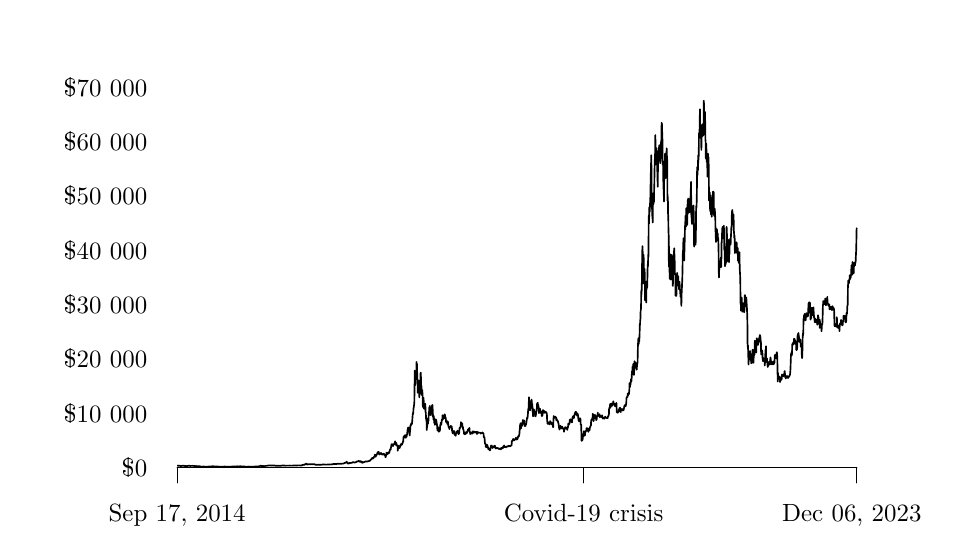
\begin{tikzpicture}[x=1pt,y=1pt]
\definecolor{fillColor}{RGB}{255,255,255}
\path[use as bounding box,fill=fillColor,fill opacity=0.00] (0,0) rectangle (325.21,180.67);
\begin{scope}
\path[clip] ( 54.00, 21.60) rectangle (303.62,159.07);
\definecolor{drawColor}{RGB}{0,0,0}

\path[draw=drawColor,line width= 0.6pt,line join=round,line cap=round] ( 54.00, 22.50) --
	( 54.07, 22.43) --
	( 54.15, 22.38) --
	( 54.22, 22.40) --
	( 54.29, 22.38) --
	( 54.36, 22.39) --
	( 54.44, 22.46) --
	( 54.51, 22.43) --
	( 54.58, 22.41) --
	( 54.66, 22.39) --
	( 54.73, 22.38) --
	( 54.80, 22.34) --
	( 54.88, 22.34) --
	( 54.95, 22.36) --
	( 55.02, 22.35) --
	( 55.09, 22.34) --
	( 55.17, 22.31) --
	( 55.24, 22.25) --
	( 55.31, 22.23) --
	( 55.39, 22.25) --
	( 55.46, 22.26) --
	( 55.53, 22.29) --
	( 55.60, 22.32) --
	( 55.68, 22.31) --
	( 55.75, 22.31) --
	( 55.82, 22.34) --
	( 55.90, 22.37) --
	( 55.97, 22.39) --
	( 56.04, 22.38) --
	( 56.12, 22.35) --
	( 56.19, 22.35) --
	( 56.26, 22.37) --
	( 56.33, 22.37) --
	( 56.41, 22.35) --
	( 56.48, 22.36) --
	( 56.55, 22.35) --
	( 56.63, 22.30) --
	( 56.70, 22.30) --
	( 56.77, 22.28) --
	( 56.84, 22.30) --
	( 56.92, 22.29) --
	( 56.99, 22.30) --
	( 57.06, 22.26) --
	( 57.14, 22.28) --
	( 57.21, 22.26) --
	( 57.28, 22.24) --
	( 57.36, 22.24) --
	( 57.43, 22.24) --
	( 57.50, 22.25) --
	( 57.57, 22.27) --
	( 57.65, 22.29) --
	( 57.72, 22.27) --
	( 57.79, 22.28) --
	( 57.87, 22.31) --
	( 57.94, 22.32) --
	( 58.01, 22.32) --
	( 58.08, 22.43) --
	( 58.16, 22.43) --
	( 58.23, 22.38) --
	( 58.30, 22.34) --
	( 58.38, 22.36) --
	( 58.45, 22.36) --
	( 58.52, 22.34) --
	( 58.60, 22.35) --
	( 58.67, 22.30) --
	( 58.74, 22.29) --
	( 58.81, 22.29) --
	( 58.89, 22.32) --
	( 58.96, 22.34) --
	( 59.03, 22.34) --
	( 59.11, 22.32) --
	( 59.18, 22.33) --
	( 59.25, 22.34) --
	( 59.32, 22.34) --
	( 59.40, 22.34) --
	( 59.47, 22.34) --
	( 59.54, 22.35) --
	( 59.62, 22.34) --
	( 59.69, 22.33) --
	( 59.76, 22.34) --
	( 59.84, 22.34) --
	( 59.91, 22.34) --
	( 59.98, 22.31) --
	( 60.05, 22.29) --
	( 60.13, 22.28) --
	( 60.20, 22.29) --
	( 60.27, 22.29) --
	( 60.35, 22.28) --
	( 60.42, 22.29) --
	( 60.49, 22.28) --
	( 60.56, 22.24) --
	( 60.64, 22.23) --
	( 60.71, 22.21) --
	( 60.78, 22.22) --
	( 60.86, 22.25) --
	( 60.93, 22.23) --
	( 61.00, 22.25) --
	( 61.08, 22.26) --
	( 61.15, 22.23) --
	( 61.22, 22.23) --
	( 61.29, 22.24) --
	( 61.37, 22.22) --
	( 61.44, 22.22) --
	( 61.51, 22.21) --
	( 61.59, 22.21) --
	( 61.66, 22.23) --
	( 61.73, 22.22) --
	( 61.81, 22.22) --
	( 61.88, 22.15) --
	( 61.95, 22.12) --
	( 62.02, 22.14) --
	( 62.10, 22.16) --
	( 62.17, 22.18) --
	( 62.24, 22.16) --
	( 62.32, 22.17) --
	( 62.39, 22.14) --
	( 62.46, 22.12) --
	( 62.53, 22.13) --
	( 62.61, 22.04) --
	( 62.68, 21.95) --
	( 62.75, 22.01) --
	( 62.83, 22.01) --
	( 62.90, 21.99) --
	( 62.97, 22.01) --
	( 63.05, 22.02) --
	( 63.12, 22.02) --
	( 63.19, 22.05) --
	( 63.26, 22.06) --
	( 63.34, 22.06) --
	( 63.41, 22.09) --
	( 63.48, 22.10) --
	( 63.56, 22.14) --
	( 63.63, 22.12) --
	( 63.70, 22.06) --
	( 63.77, 22.06) --
	( 63.85, 22.04) --
	( 63.92, 22.03) --
	( 63.99, 22.05) --
	( 64.07, 22.07) --
	( 64.14, 22.05) --
	( 64.21, 22.05) --
	( 64.29, 22.03) --
	( 64.36, 22.04) --
	( 64.43, 22.05) --
	( 64.50, 22.04) --
	( 64.58, 22.03) --
	( 64.65, 22.03) --
	( 64.72, 22.03) --
	( 64.80, 22.04) --
	( 64.87, 22.06) --
	( 64.94, 22.11) --
	( 65.01, 22.06) --
	( 65.09, 22.06) --
	( 65.16, 22.08) --
	( 65.23, 22.06) --
	( 65.31, 22.07) --
	( 65.38, 22.08) --
	( 65.45, 22.08) --
	( 65.53, 22.06) --
	( 65.60, 22.07) --
	( 65.67, 22.07) --
	( 65.74, 22.07) --
	( 65.82, 22.06) --
	( 65.89, 22.10) --
	( 65.96, 22.10) --
	( 66.04, 22.11) --
	( 66.11, 22.14) --
	( 66.18, 22.15) --
	( 66.25, 22.14) --
	( 66.33, 22.14) --
	( 66.40, 22.14) --
	( 66.47, 22.14) --
	( 66.55, 22.14) --
	( 66.62, 22.17) --
	( 66.69, 22.17) --
	( 66.77, 22.18) --
	( 66.84, 22.18) --
	( 66.91, 22.16) --
	( 66.98, 22.15) --
	( 67.06, 22.16) --
	( 67.13, 22.17) --
	( 67.20, 22.16) --
	( 67.28, 22.10) --
	( 67.35, 22.11) --
	( 67.42, 22.11) --
	( 67.49, 22.11) --
	( 67.57, 22.13) --
	( 67.64, 22.12) --
	( 67.71, 22.08) --
	( 67.79, 22.08) --
	( 67.86, 22.09) --
	( 67.93, 22.09) --
	( 68.01, 22.10) --
	( 68.08, 22.08) --
	( 68.15, 22.09) --
	( 68.22, 22.08) --
	( 68.30, 22.09) --
	( 68.37, 22.10) --
	( 68.44, 22.10) --
	( 68.52, 22.10) --
	( 68.59, 22.11) --
	( 68.66, 22.10) --
	( 68.73, 22.10) --
	( 68.81, 22.08) --
	( 68.88, 22.08) --
	( 68.95, 22.06) --
	( 69.03, 22.06) --
	( 69.10, 22.06) --
	( 69.17, 22.04) --
	( 69.25, 22.03) --
	( 69.32, 22.04) --
	( 69.39, 22.05) --
	( 69.46, 22.04) --
	( 69.54, 22.04) --
	( 69.61, 22.04) --
	( 69.68, 22.04) --
	( 69.76, 22.06) --
	( 69.83, 22.06) --
	( 69.90, 22.06) --
	( 69.97, 22.05) --
	( 70.05, 22.04) --
	( 70.12, 22.03) --
	( 70.19, 22.05) --
	( 70.27, 22.04) --
	( 70.34, 22.04) --
	( 70.41, 22.06) --
	( 70.49, 22.06) --
	( 70.56, 22.06) --
	( 70.63, 22.07) --
	( 70.70, 22.07) --
	( 70.78, 22.06) --
	( 70.85, 22.05) --
	( 70.92, 22.07) --
	( 71.00, 22.08) --
	( 71.07, 22.07) --
	( 71.14, 22.07) --
	( 71.21, 22.08) --
	( 71.29, 22.07) --
	( 71.36, 22.06) --
	( 71.43, 22.07) --
	( 71.51, 22.07) --
	( 71.58, 22.06) --
	( 71.65, 22.07) --
	( 71.73, 22.06) --
	( 71.80, 22.06) --
	( 71.87, 22.06) --
	( 71.94, 22.06) --
	( 72.02, 22.07) --
	( 72.09, 22.07) --
	( 72.16, 22.07) --
	( 72.24, 22.07) --
	( 72.31, 22.07) --
	( 72.38, 22.07) --
	( 72.45, 22.07) --
	( 72.53, 22.07) --
	( 72.60, 22.06) --
	( 72.67, 22.05) --
	( 72.75, 22.04) --
	( 72.82, 22.04) --
	( 72.89, 22.04) --
	( 72.97, 22.04) --
	( 73.04, 22.04) --
	( 73.11, 22.04) --
	( 73.18, 22.04) --
	( 73.26, 22.05) --
	( 73.33, 22.05) --
	( 73.40, 22.05) --
	( 73.48, 22.05) --
	( 73.55, 22.05) --
	( 73.62, 22.06) --
	( 73.69, 22.06) --
	( 73.77, 22.07) --
	( 73.84, 22.09) --
	( 73.91, 22.09) --
	( 73.99, 22.09) --
	( 74.06, 22.08) --
	( 74.13, 22.08) --
	( 74.21, 22.08) --
	( 74.28, 22.09) --
	( 74.35, 22.08) --
	( 74.42, 22.07) --
	( 74.50, 22.08) --
	( 74.57, 22.08) --
	( 74.64, 22.09) --
	( 74.72, 22.09) --
	( 74.79, 22.10) --
	( 74.86, 22.12) --
	( 74.93, 22.11) --
	( 75.01, 22.10) --
	( 75.08, 22.10) --
	( 75.15, 22.11) --
	( 75.23, 22.13) --
	( 75.30, 22.13) --
	( 75.37, 22.12) --
	( 75.45, 22.13) --
	( 75.52, 22.13) --
	( 75.59, 22.16) --
	( 75.66, 22.18) --
	( 75.74, 22.21) --
	( 75.81, 22.17) --
	( 75.88, 22.16) --
	( 75.96, 22.16) --
	( 76.03, 22.15) --
	( 76.10, 22.15) --
	( 76.18, 22.14) --
	( 76.25, 22.14) --
	( 76.32, 22.15) --
	( 76.39, 22.14) --
	( 76.47, 22.14) --
	( 76.54, 22.14) --
	( 76.61, 22.17) --
	( 76.69, 22.17) --
	( 76.76, 22.17) --
	( 76.83, 22.18) --
	( 76.90, 22.18) --
	( 76.98, 22.17) --
	( 77.05, 22.17) --
	( 77.12, 22.16) --
	( 77.20, 22.15) --
	( 77.27, 22.16) --
	( 77.34, 22.15) --
	( 77.42, 22.16) --
	( 77.49, 22.15) --
	( 77.56, 22.15) --
	( 77.63, 22.15) --
	( 77.71, 22.11) --
	( 77.78, 22.12) --
	( 77.85, 22.12) --
	( 77.93, 22.13) --
	( 78.00, 22.12) --
	( 78.07, 22.12) --
	( 78.14, 22.12) --
	( 78.22, 22.11) --
	( 78.29, 22.11) --
	( 78.36, 22.11) --
	( 78.44, 22.01) --
	( 78.51, 22.05) --
	( 78.58, 22.06) --
	( 78.66, 22.06) --
	( 78.73, 22.05) --
	( 78.80, 22.05) --
	( 78.87, 22.01) --
	( 78.95, 22.04) --
	( 79.02, 22.04) --
	( 79.09, 22.04) --
	( 79.17, 22.05) --
	( 79.24, 22.05) --
	( 79.31, 22.05) --
	( 79.38, 22.05) --
	( 79.46, 22.05) --
	( 79.53, 22.05) --
	( 79.60, 22.05) --
	( 79.68, 22.05) --
	( 79.75, 22.06) --
	( 79.82, 22.07) --
	( 79.90, 22.07) --
	( 79.97, 22.08) --
	( 80.04, 22.07) --
	( 80.11, 22.07) --
	( 80.19, 22.07) --
	( 80.26, 22.06) --
	( 80.33, 22.05) --
	( 80.41, 22.05) --
	( 80.48, 22.05) --
	( 80.55, 22.05) --
	( 80.62, 22.05) --
	( 80.70, 22.06) --
	( 80.77, 22.05) --
	( 80.84, 22.05) --
	( 80.92, 22.05) --
	( 80.99, 22.05) --
	( 81.06, 22.05) --
	( 81.14, 22.06) --
	( 81.21, 22.06) --
	( 81.28, 22.06) --
	( 81.35, 22.06) --
	( 81.43, 22.07) --
	( 81.50, 22.06) --
	( 81.57, 22.06) --
	( 81.65, 22.07) --
	( 81.72, 22.07) --
	( 81.79, 22.07) --
	( 81.86, 22.07) --
	( 81.94, 22.07) --
	( 82.01, 22.08) --
	( 82.08, 22.08) --
	( 82.16, 22.08) --
	( 82.23, 22.08) --
	( 82.30, 22.08) --
	( 82.38, 22.09) --
	( 82.45, 22.08) --
	( 82.52, 22.09) --
	( 82.59, 22.09) --
	( 82.67, 22.10) --
	( 82.74, 22.12) --
	( 82.81, 22.13) --
	( 82.89, 22.11) --
	( 82.96, 22.12) --
	( 83.03, 22.13) --
	( 83.10, 22.12) --
	( 83.18, 22.14) --
	( 83.25, 22.14) --
	( 83.32, 22.15) --
	( 83.40, 22.16) --
	( 83.47, 22.16) --
	( 83.54, 22.18) --
	( 83.62, 22.20) --
	( 83.69, 22.22) --
	( 83.76, 22.24) --
	( 83.83, 22.22) --
	( 83.91, 22.24) --
	( 83.98, 22.31) --
	( 84.05, 22.39) --
	( 84.13, 22.41) --
	( 84.20, 22.36) --
	( 84.27, 22.34) --
	( 84.34, 22.36) --
	( 84.42, 22.33) --
	( 84.49, 22.35) --
	( 84.56, 22.26) --
	( 84.64, 22.21) --
	( 84.71, 22.26) --
	( 84.78, 22.26) --
	( 84.86, 22.25) --
	( 84.93, 22.23) --
	( 85.00, 22.25) --
	( 85.07, 22.26) --
	( 85.15, 22.26) --
	( 85.22, 22.24) --
	( 85.29, 22.23) --
	( 85.37, 22.24) --
	( 85.44, 22.24) --
	( 85.51, 22.23) --
	( 85.58, 22.23) --
	( 85.66, 22.24) --
	( 85.73, 22.29) --
	( 85.80, 22.30) --
	( 85.88, 22.30) --
	( 85.95, 22.33) --
	( 86.02, 22.34) --
	( 86.10, 22.31) --
	( 86.17, 22.31) --
	( 86.24, 22.31) --
	( 86.31, 22.31) --
	( 86.39, 22.36) --
	( 86.46, 22.36) --
	( 86.53, 22.38) --
	( 86.61, 22.42) --
	( 86.68, 22.42) --
	( 86.75, 22.42) --
	( 86.82, 22.49) --
	( 86.90, 22.45) --
	( 86.97, 22.45) --
	( 87.04, 22.47) --
	( 87.12, 22.51) --
	( 87.19, 22.49) --
	( 87.26, 22.50) --
	( 87.34, 22.51) --
	( 87.41, 22.51) --
	( 87.48, 22.47) --
	( 87.55, 22.46) --
	( 87.63, 22.46) --
	( 87.70, 22.47) --
	( 87.77, 22.49) --
	( 87.85, 22.49) --
	( 87.92, 22.42) --
	( 87.99, 22.43) --
	( 88.06, 22.43) --
	( 88.14, 22.45) --
	( 88.21, 22.44) --
	( 88.28, 22.45) --
	( 88.36, 22.45) --
	( 88.43, 22.45) --
	( 88.50, 22.44) --
	( 88.58, 22.45) --
	( 88.65, 22.45) --
	( 88.72, 22.44) --
	( 88.79, 22.50) --
	( 88.87, 22.49) --
	( 88.94, 22.48) --
	( 89.01, 22.48) --
	( 89.09, 22.48) --
	( 89.16, 22.46) --
	( 89.23, 22.45) --
	( 89.30, 22.45) --
	( 89.38, 22.32) --
	( 89.45, 22.36) --
	( 89.52, 22.35) --
	( 89.60, 22.36) --
	( 89.67, 22.35) --
	( 89.74, 22.43) --
	( 89.82, 22.41) --
	( 89.89, 22.35) --
	( 89.96, 22.36) --
	( 90.03, 22.39) --
	( 90.11, 22.37) --
	( 90.18, 22.37) --
	( 90.25, 22.38) --
	( 90.33, 22.35) --
	( 90.40, 22.35) --
	( 90.47, 22.34) --
	( 90.55, 22.32) --
	( 90.62, 22.33) --
	( 90.69, 22.34) --
	( 90.76, 22.33) --
	( 90.84, 22.37) --
	( 90.91, 22.36) --
	( 90.98, 22.34) --
	( 91.06, 22.34) --
	( 91.13, 22.33) --
	( 91.20, 22.34) --
	( 91.27, 22.35) --
	( 91.35, 22.35) --
	( 91.42, 22.35) --
	( 91.49, 22.37) --
	( 91.57, 22.40) --
	( 91.64, 22.39) --
	( 91.71, 22.40) --
	( 91.79, 22.42) --
	( 91.86, 22.43) --
	( 91.93, 22.43) --
	( 92.00, 22.46) --
	( 92.08, 22.46) --
	( 92.15, 22.46) --
	( 92.22, 22.43) --
	( 92.30, 22.43) --
	( 92.37, 22.43) --
	( 92.44, 22.45) --
	( 92.51, 22.45) --
	( 92.59, 22.45) --
	( 92.66, 22.46) --
	( 92.73, 22.45) --
	( 92.81, 22.43) --
	( 92.88, 22.43) --
	( 92.95, 22.41) --
	( 93.03, 22.39) --
	( 93.10, 22.40) --
	( 93.17, 22.41) --
	( 93.24, 22.41) --
	( 93.32, 22.41) --
	( 93.39, 22.42) --
	( 93.46, 22.43) --
	( 93.54, 22.41) --
	( 93.61, 22.41) --
	( 93.68, 22.42) --
	( 93.75, 22.42) --
	( 93.83, 22.42) --
	( 93.90, 22.43) --
	( 93.97, 22.40) --
	( 94.05, 22.41) --
	( 94.12, 22.41) --
	( 94.19, 22.41) --
	( 94.27, 22.42) --
	( 94.34, 22.42) --
	( 94.41, 22.42) --
	( 94.48, 22.42) --
	( 94.56, 22.42) --
	( 94.63, 22.44) --
	( 94.70, 22.43) --
	( 94.78, 22.42) --
	( 94.85, 22.41) --
	( 94.92, 22.42) --
	( 94.99, 22.42) --
	( 95.07, 22.43) --
	( 95.14, 22.43) --
	( 95.21, 22.43) --
	( 95.29, 22.43) --
	( 95.36, 22.43) --
	( 95.43, 22.43) --
	( 95.51, 22.43) --
	( 95.58, 22.42) --
	( 95.65, 22.43) --
	( 95.72, 22.43) --
	( 95.80, 22.44) --
	( 95.87, 22.43) --
	( 95.94, 22.43) --
	( 96.02, 22.44) --
	( 96.09, 22.45) --
	( 96.16, 22.44) --
	( 96.23, 22.44) --
	( 96.31, 22.46) --
	( 96.38, 22.47) --
	( 96.45, 22.48) --
	( 96.53, 22.48) --
	( 96.60, 22.48) --
	( 96.67, 22.50) --
	( 96.75, 22.51) --
	( 96.82, 22.52) --
	( 96.89, 22.47) --
	( 96.96, 22.48) --
	( 97.04, 22.49) --
	( 97.11, 22.48) --
	( 97.18, 22.49) --
	( 97.26, 22.47) --
	( 97.33, 22.48) --
	( 97.40, 22.48) --
	( 97.47, 22.48) --
	( 97.55, 22.50) --
	( 97.62, 22.50) --
	( 97.69, 22.50) --
	( 97.77, 22.50) --
	( 97.84, 22.49) --
	( 97.91, 22.49) --
	( 97.99, 22.49) --
	( 98.06, 22.49) --
	( 98.13, 22.49) --
	( 98.20, 22.50) --
	( 98.28, 22.49) --
	( 98.35, 22.49) --
	( 98.42, 22.49) --
	( 98.50, 22.46) --
	( 98.57, 22.47) --
	( 98.64, 22.47) --
	( 98.71, 22.46) --
	( 98.79, 22.47) --
	( 98.86, 22.48) --
	( 98.93, 22.48) --
	( 99.01, 22.49) --
	( 99.08, 22.53) --
	( 99.15, 22.64) --
	( 99.23, 22.63) --
	( 99.30, 22.65) --
	( 99.37, 22.64) --
	( 99.44, 22.65) --
	( 99.52, 22.66) --
	( 99.59, 22.72) --
	( 99.66, 22.72) --
	( 99.74, 22.73) --
	( 99.81, 22.75) --
	( 99.88, 22.73) --
	( 99.95, 22.74) --
	(100.03, 22.73) --
	(100.10, 22.73) --
	(100.17, 22.79) --
	(100.25, 22.92) --
	(100.32, 22.98) --
	(100.39, 22.95) --
	(100.47, 22.96) --
	(100.54, 23.10) --
	(100.61, 23.07) --
	(100.68, 23.09) --
	(100.76, 23.10) --
	(100.83, 23.05) --
	(100.90, 22.91) --
	(100.98, 22.77) --
	(101.05, 22.83) --
	(101.12, 22.91) --
	(101.19, 22.91) --
	(101.27, 22.84) --
	(101.34, 22.89) --
	(101.41, 22.87) --
	(101.49, 22.86) --
	(101.56, 22.92) --
	(101.63, 22.93) --
	(101.71, 22.98) --
	(101.78, 22.89) --
	(101.85, 22.94) --
	(101.92, 22.92) --
	(102.00, 22.93) --
	(102.07, 22.86) --
	(102.14, 22.91) --
	(102.22, 22.88) --
	(102.29, 22.88) --
	(102.36, 22.87) --
	(102.43, 22.91) --
	(102.51, 22.89) --
	(102.58, 22.89) --
	(102.65, 22.90) --
	(102.73, 22.90) --
	(102.80, 22.93) --
	(102.87, 22.92) --
	(102.95, 22.92) --
	(103.02, 22.91) --
	(103.09, 22.91) --
	(103.16, 22.88) --
	(103.24, 22.89) --
	(103.31, 22.90) --
	(103.38, 22.88) --
	(103.46, 22.88) --
	(103.53, 22.89) --
	(103.60, 22.89) --
	(103.67, 22.89) --
	(103.75, 22.89) --
	(103.82, 22.83) --
	(103.89, 22.79) --
	(103.97, 22.68) --
	(104.04, 22.71) --
	(104.11, 22.74) --
	(104.19, 22.73) --
	(104.26, 22.75) --
	(104.33, 22.76) --
	(104.40, 22.76) --
	(104.48, 22.75) --
	(104.55, 22.76) --
	(104.62, 22.76) --
	(104.70, 22.75) --
	(104.77, 22.75) --
	(104.84, 22.72) --
	(104.92, 22.71) --
	(104.99, 22.73) --
	(105.06, 22.73) --
	(105.13, 22.73) --
	(105.21, 22.73) --
	(105.28, 22.74) --
	(105.35, 22.74) --
	(105.43, 22.75) --
	(105.50, 22.75) --
	(105.57, 22.74) --
	(105.64, 22.73) --
	(105.72, 22.74) --
	(105.79, 22.72) --
	(105.86, 22.73) --
	(105.94, 22.73) --
	(106.01, 22.73) --
	(106.08, 22.73) --
	(106.16, 22.72) --
	(106.23, 22.73) --
	(106.30, 22.77) --
	(106.37, 22.80) --
	(106.45, 22.79) --
	(106.52, 22.80) --
	(106.59, 22.81) --
	(106.67, 22.83) --
	(106.74, 22.82) --
	(106.81, 22.82) --
	(106.88, 22.79) --
	(106.96, 22.79) --
	(107.03, 22.80) --
	(107.10, 22.80) --
	(107.18, 22.79) --
	(107.25, 22.79) --
	(107.32, 22.79) --
	(107.40, 22.80) --
	(107.47, 22.80) --
	(107.54, 22.79) --
	(107.61, 22.77) --
	(107.69, 22.77) --
	(107.76, 22.78) --
	(107.83, 22.78) --
	(107.91, 22.78) --
	(107.98, 22.79) --
	(108.05, 22.79) --
	(108.12, 22.79) --
	(108.20, 22.79) --
	(108.27, 22.80) --
	(108.34, 22.81) --
	(108.42, 22.80) --
	(108.49, 22.80) --
	(108.56, 22.80) --
	(108.64, 22.80) --
	(108.71, 22.80) --
	(108.78, 22.81) --
	(108.85, 22.82) --
	(108.93, 22.81) --
	(109.00, 22.82) --
	(109.07, 22.86) --
	(109.15, 22.85) --
	(109.22, 22.85) --
	(109.29, 22.86) --
	(109.36, 22.85) --
	(109.44, 22.86) --
	(109.51, 22.86) --
	(109.58, 22.85) --
	(109.66, 22.84) --
	(109.73, 22.84) --
	(109.80, 22.84) --
	(109.88, 22.89) --
	(109.95, 22.89) --
	(110.02, 22.88) --
	(110.09, 22.89) --
	(110.17, 22.93) --
	(110.24, 22.95) --
	(110.31, 22.95) --
	(110.39, 23.00) --
	(110.46, 22.98) --
	(110.53, 22.98) --
	(110.60, 23.03) --
	(110.68, 23.05) --
	(110.75, 22.95) --
	(110.82, 22.98) --
	(110.90, 22.98) --
	(110.97, 23.00) --
	(111.04, 22.98) --
	(111.12, 22.99) --
	(111.19, 23.02) --
	(111.26, 23.01) --
	(111.33, 23.01) --
	(111.41, 22.98) --
	(111.48, 22.98) --
	(111.55, 22.98) --
	(111.63, 23.00) --
	(111.70, 23.06) --
	(111.77, 23.06) --
	(111.84, 23.08) --
	(111.92, 23.08) --
	(111.99, 23.04) --
	(112.06, 23.05) --
	(112.14, 23.08) --
	(112.21, 23.06) --
	(112.28, 23.05) --
	(112.36, 23.06) --
	(112.43, 23.04) --
	(112.50, 23.04) --
	(112.57, 23.05) --
	(112.65, 23.04) --
	(112.72, 23.06) --
	(112.79, 23.09) --
	(112.87, 23.13) --
	(112.94, 23.11) --
	(113.01, 23.12) --
	(113.08, 23.09) --
	(113.16, 23.10) --
	(113.23, 23.11) --
	(113.30, 23.11) --
	(113.38, 23.12) --
	(113.45, 23.12) --
	(113.52, 23.11) --
	(113.60, 23.13) --
	(113.67, 23.13) --
	(113.74, 23.13) --
	(113.81, 23.13) --
	(113.89, 23.14) --
	(113.96, 23.15) --
	(114.03, 23.15) --
	(114.11, 23.16) --
	(114.18, 23.17) --
	(114.25, 23.24) --
	(114.32, 23.30) --
	(114.40, 23.41) --
	(114.47, 23.37) --
	(114.54, 23.36) --
	(114.62, 23.38) --
	(114.69, 23.43) --
	(114.76, 23.52) --
	(114.84, 23.51) --
	(114.91, 23.49) --
	(114.98, 23.49) --
	(115.05, 23.56) --
	(115.13, 23.61) --
	(115.20, 23.65) --
	(115.27, 23.87) --
	(115.35, 23.59) --
	(115.42, 23.37) --
	(115.49, 23.38) --
	(115.56, 23.39) --
	(115.64, 23.37) --
	(115.71, 23.38) --
	(115.78, 23.13) --
	(115.86, 23.18) --
	(115.93, 23.22) --
	(116.00, 23.21) --
	(116.08, 23.21) --
	(116.15, 23.23) --
	(116.22, 23.38) --
	(116.29, 23.34) --
	(116.37, 23.37) --
	(116.44, 23.36) --
	(116.51, 23.41) --
	(116.59, 23.42) --
	(116.66, 23.41) --
	(116.73, 23.35) --
	(116.80, 23.37) --
	(116.88, 23.40) --
	(116.95, 23.41) --
	(117.02, 23.41) --
	(117.10, 23.41) --
	(117.17, 23.41) --
	(117.24, 23.51) --
	(117.32, 23.54) --
	(117.39, 23.59) --
	(117.46, 23.62) --
	(117.53, 23.65) --
	(117.61, 23.62) --
	(117.68, 23.64) --
	(117.75, 23.68) --
	(117.83, 23.69) --
	(117.90, 23.55) --
	(117.97, 23.54) --
	(118.04, 23.57) --
	(118.12, 23.56) --
	(118.19, 23.55) --
	(118.26, 23.57) --
	(118.34, 23.58) --
	(118.41, 23.62) --
	(118.48, 23.65) --
	(118.56, 23.67) --
	(118.63, 23.66) --
	(118.70, 23.72) --
	(118.77, 23.79) --
	(118.85, 23.79) --
	(118.92, 23.89) --
	(118.99, 23.91) --
	(119.07, 23.85) --
	(119.14, 23.89) --
	(119.21, 23.92) --
	(119.29, 23.92) --
	(119.36, 24.00) --
	(119.43, 24.06) --
	(119.50, 24.10) --
	(119.58, 24.07) --
	(119.65, 24.09) --
	(119.72, 24.10) --
	(119.80, 24.00) --
	(119.87, 23.86) --
	(119.94, 23.93) --
	(120.01, 23.79) --
	(120.09, 23.91) --
	(120.16, 24.00) --
	(120.23, 24.02) --
	(120.31, 24.04) --
	(120.38, 24.05) --
	(120.45, 23.93) --
	(120.53, 23.76) --
	(120.60, 23.51) --
	(120.67, 23.64) --
	(120.74, 23.67) --
	(120.82, 23.80) --
	(120.89, 23.66) --
	(120.96, 23.64) --
	(121.04, 23.44) --
	(121.11, 23.51) --
	(121.18, 23.50) --
	(121.25, 23.65) --
	(121.33, 23.66) --
	(121.40, 23.64) --
	(121.47, 23.62) --
	(121.55, 23.70) --
	(121.62, 23.72) --
	(121.69, 23.76) --
	(121.77, 23.85) --
	(121.84, 23.83) --
	(121.91, 23.81) --
	(121.98, 23.92) --
	(122.06, 23.91) --
	(122.13, 23.91) --
	(122.20, 23.93) --
	(122.28, 23.93) --
	(122.35, 23.97) --
	(122.42, 23.96) --
	(122.49, 23.90) --
	(122.57, 23.89) --
	(122.64, 23.90) --
	(122.71, 23.92) --
	(122.79, 23.94) --
	(122.86, 23.98) --
	(122.93, 23.98) --
	(123.01, 24.01) --
	(123.08, 24.00) --
	(123.15, 24.02) --
	(123.22, 23.97) --
	(123.30, 24.06) --
	(123.37, 24.09) --
	(123.44, 24.12) --
	(123.52, 24.19) --
	(123.59, 24.19) --
	(123.66, 24.20) --
	(123.73, 24.25) --
	(123.81, 24.39) --
	(123.88, 24.45) --
	(123.95, 24.53) --
	(124.03, 24.62) --
	(124.10, 24.65) --
	(124.17, 24.70) --
	(124.25, 24.74) --
	(124.32, 24.98) --
	(124.39, 25.05) --
	(124.46, 25.11) --
	(124.54, 25.23) --
	(124.61, 24.99) --
	(124.68, 25.14) --
	(124.76, 25.15) --
	(124.83, 25.01) --
	(124.90, 25.01) --
	(124.97, 25.21) --
	(125.05, 25.31) --
	(125.12, 25.50) --
	(125.19, 25.69) --
	(125.27, 25.61) --
	(125.34, 25.87) --
	(125.41, 26.16) --
	(125.49, 26.40) --
	(125.56, 26.13) --
	(125.63, 25.93) --
	(125.70, 25.60) --
	(125.78, 25.83) --
	(125.85, 26.03) --
	(125.92, 25.87) --
	(126.00, 26.09) --
	(126.07, 26.33) --
	(126.14, 26.49) --
	(126.21, 26.54) --
	(126.29, 26.53) --
	(126.36, 26.88) --
	(126.43, 27.22) --
	(126.51, 26.97) --
	(126.58, 27.11) --
	(126.65, 27.15) --
	(126.73, 27.39) --
	(126.80, 27.41) --
	(126.87, 26.82) --
	(126.94, 26.94) --
	(127.02, 26.52) --
	(127.09, 26.44) --
	(127.16, 26.55) --
	(127.24, 26.82) --
	(127.31, 26.60) --
	(127.38, 26.69) --
	(127.45, 26.95) --
	(127.53, 26.88) --
	(127.60, 26.91) --
	(127.67, 26.99) --
	(127.75, 26.72) --
	(127.82, 26.69) --
	(127.89, 26.47) --
	(127.97, 26.61) --
	(128.04, 26.66) --
	(128.11, 26.59) --
	(128.18, 26.47) --
	(128.26, 26.38) --
	(128.33, 26.52) --
	(128.40, 26.64) --
	(128.48, 26.71) --
	(128.55, 26.71) --
	(128.62, 26.72) --
	(128.69, 26.55) --
	(128.77, 26.65) --
	(128.84, 26.55) --
	(128.91, 26.26) --
	(128.99, 26.19) --
	(129.06, 26.31) --
	(129.13, 26.23) --
	(129.21, 25.99) --
	(129.28, 25.53) --
	(129.35, 25.39) --
	(129.42, 25.98) --
	(129.50, 26.15) --
	(129.57, 26.06) --
	(129.64, 27.13) --
	(129.72, 26.84) --
	(129.79, 27.12) --
	(129.86, 26.96) --
	(129.93, 27.01) --
	(130.01, 26.66) --
	(130.08, 26.57) --
	(130.15, 26.85) --
	(130.23, 27.12) --
	(130.30, 26.95) --
	(130.37, 27.01) --
	(130.45, 27.25) --
	(130.52, 26.94) --
	(130.59, 26.92) --
	(130.66, 27.11) --
	(130.74, 27.29) --
	(130.81, 27.99) --
	(130.88, 27.91) --
	(130.96, 28.24) --
	(131.03, 28.32) --
	(131.10, 28.16) --
	(131.17, 28.24) --
	(131.25, 28.77) --
	(131.32, 29.23) --
	(131.39, 29.60) --
	(131.47, 30.09) --
	(131.54, 29.81) --
	(131.61, 30.20) --
	(131.69, 30.11) --
	(131.76, 29.77) --
	(131.83, 29.84) --
	(131.90, 29.63) --
	(131.98, 29.46) --
	(132.05, 29.65) --
	(132.12, 29.75) --
	(132.20, 30.11) --
	(132.27, 30.19) --
	(132.34, 30.15) --
	(132.41, 30.21) --
	(132.49, 30.21) --
	(132.56, 30.59) --
	(132.63, 30.57) --
	(132.71, 30.84) --
	(132.78, 31.21) --
	(132.85, 30.59) --
	(132.93, 30.60) --
	(133.00, 29.92) --
	(133.07, 30.20) --
	(133.14, 30.63) --
	(133.22, 30.63) --
	(133.29, 29.90) --
	(133.36, 29.90) --
	(133.44, 29.70) --
	(133.51, 29.77) --
	(133.58, 29.71) --
	(133.66, 29.23) --
	(133.73, 27.80) --
	(133.80, 28.74) --
	(133.87, 28.72) --
	(133.95, 28.64) --
	(134.02, 29.58) --
	(134.09, 29.31) --
	(134.17, 29.27) --
	(134.24, 28.73) --
	(134.31, 28.73) --
	(134.38, 29.05) --
	(134.46, 28.83) --
	(134.53, 29.31) --
	(134.60, 29.24) --
	(134.68, 29.85) --
	(134.75, 29.80) --
	(134.82, 29.78) --
	(134.90, 30.12) --
	(134.97, 30.25) --
	(135.04, 30.26) --
	(135.11, 30.08) --
	(135.19, 29.91) --
	(135.26, 30.10) --
	(135.33, 30.18) --
	(135.41, 30.29) --
	(135.48, 30.65) --
	(135.55, 30.97) --
	(135.62, 30.99) --
	(135.70, 31.08) --
	(135.77, 32.30) --
	(135.84, 32.69) --
	(135.92, 33.05) --
	(135.99, 32.75) --
	(136.06, 32.84) --
	(136.14, 32.61) --
	(136.21, 32.58) --
	(136.28, 32.81) --
	(136.35, 33.41) --
	(136.43, 33.45) --
	(136.50, 33.40) --
	(136.57, 33.25) --
	(136.65, 32.45) --
	(136.72, 32.89) --
	(136.79, 33.20) --
	(136.86, 32.95) --
	(136.94, 32.90) --
	(137.01, 33.69) --
	(137.08, 33.64) --
	(137.16, 34.30) --
	(137.23, 34.89) --
	(137.30, 35.50) --
	(137.38, 35.76) --
	(137.45, 36.09) --
	(137.52, 36.15) --
	(137.59, 35.39) --
	(137.67, 35.63) --
	(137.74, 36.25) --
	(137.81, 35.63) --
	(137.89, 34.60) --
	(137.96, 34.09) --
	(138.03, 33.29) --
	(138.10, 34.48) --
	(138.18, 34.63) --
	(138.25, 35.97) --
	(138.32, 37.06) --
	(138.40, 36.74) --
	(138.47, 36.90) --
	(138.54, 37.38) --
	(138.62, 37.71) --
	(138.69, 37.45) --
	(138.76, 37.81) --
	(138.83, 37.39) --
	(138.91, 37.81) --
	(138.98, 38.86) --
	(139.05, 39.92) --
	(139.13, 40.88) --
	(139.20, 41.35) --
	(139.27, 41.02) --
	(139.34, 41.70) --
	(139.42, 43.16) --
	(139.49, 43.35) --
	(139.56, 43.84) --
	(139.64, 44.49) --
	(139.71, 45.00) --
	(139.78, 49.67) --
	(139.86, 56.75) --
	(139.93, 54.14) --
	(140.00, 51.41) --
	(140.07, 51.95) --
	(140.15, 54.86) --
	(140.22, 55.80) --
	(140.29, 53.82) --
	(140.37, 54.13) --
	(140.44, 56.38) --
	(140.51, 59.89) --
	(140.58, 59.19) --
	(140.66, 59.14) --
	(140.73, 56.51) --
	(140.80, 54.25) --
	(140.88, 52.64) --
	(140.95, 48.76) --
	(141.02, 50.47) --
	(141.10, 48.95) --
	(141.17, 49.15) --
	(141.24, 53.22) --
	(141.31, 52.71) --
	(141.39, 50.29) --
	(141.46, 50.38) --
	(141.53, 47.04) --
	(141.61, 49.40) --
	(141.68, 48.42) --
	(141.75, 51.02) --
	(141.82, 51.45) --
	(141.90, 52.24) --
	(141.97, 55.83) --
	(142.04, 56.02) --
	(142.12, 53.96) --
	(142.19, 51.39) --
	(142.26, 50.26) --
	(142.34, 51.01) --
	(142.41, 47.93) --
	(142.48, 49.06) --
	(142.55, 49.80) --
	(142.63, 48.65) --
	(142.70, 48.74) --
	(142.77, 44.17) --
	(142.85, 43.57) --
	(142.92, 44.14) --
	(142.99, 44.40) --
	(143.06, 46.93) --
	(143.14, 44.38) --
	(143.21, 43.07) --
	(143.28, 42.94) --
	(143.36, 43.91) --
	(143.43, 43.71) --
	(143.50, 43.54) --
	(143.58, 44.07) --
	(143.65, 44.75) --
	(143.72, 43.79) --
	(143.79, 41.45) --
	(143.87, 41.67) --
	(143.94, 39.61) --
	(144.01, 38.94) --
	(144.09, 39.62) --
	(144.16, 37.86) --
	(144.23, 35.26) --
	(144.30, 36.83) --
	(144.38, 36.57) --
	(144.45, 37.83) --
	(144.52, 38.76) --
	(144.60, 38.53) --
	(144.67, 37.57) --
	(144.74, 39.13) --
	(144.82, 38.49) --
	(144.89, 40.25) --
	(144.96, 41.57) --
	(145.03, 41.70) --
	(145.11, 43.42) --
	(145.18, 42.32) --
	(145.25, 43.65) --
	(145.33, 44.00) --
	(145.40, 42.60) --
	(145.47, 41.25) --
	(145.54, 41.83) --
	(145.62, 40.87) --
	(145.69, 40.58) --
	(145.76, 41.96) --
	(145.84, 42.66) --
	(145.91, 42.02) --
	(145.98, 43.11) --
	(146.06, 43.37) --
	(146.13, 44.16) --
	(146.20, 44.21) --
	(146.27, 44.33) --
	(146.35, 42.77) --
	(146.42, 41.17) --
	(146.49, 40.05) --
	(146.57, 39.94) --
	(146.64, 39.01) --
	(146.71, 40.41) --
	(146.79, 39.68) --
	(146.86, 39.66) --
	(146.93, 37.84) --
	(147.00, 37.90) --
	(147.08, 37.98) --
	(147.15, 37.15) --
	(147.22, 37.75) --
	(147.30, 38.55) --
	(147.37, 39.11) --
	(147.44, 39.14) --
	(147.51, 38.74) --
	(147.59, 39.04) --
	(147.66, 38.62) --
	(147.73, 38.29) --
	(147.81, 37.72) --
	(147.88, 36.98) --
	(147.95, 37.22) --
	(148.03, 35.67) --
	(148.10, 35.13) --
	(148.17, 35.30) --
	(148.24, 35.04) --
	(148.32, 35.51) --
	(148.39, 36.24) --
	(148.46, 35.06) --
	(148.54, 34.98) --
	(148.61, 34.63) --
	(148.68, 35.17) --
	(148.75, 35.39) --
	(148.83, 34.90) --
	(148.90, 35.02) --
	(148.97, 35.29) --
	(149.05, 37.09) --
	(149.12, 37.11) --
	(149.19, 37.28) --
	(149.27, 37.96) --
	(149.34, 37.43) --
	(149.41, 37.12) --
	(149.48, 37.63) --
	(149.56, 37.89) --
	(149.63, 38.97) --
	(149.70, 39.07) --
	(149.78, 38.89) --
	(149.85, 39.14) --
	(149.92, 40.65) --
	(149.99, 38.97) --
	(150.07, 39.83) --
	(150.14, 39.25) --
	(150.21, 39.96) --
	(150.29, 40.10) --
	(150.36, 39.75) --
	(150.43, 39.51) --
	(150.51, 39.74) --
	(150.58, 40.74) --
	(150.65, 40.65) --
	(150.72, 40.96) --
	(150.80, 40.56) --
	(150.87, 40.01) --
	(150.94, 39.74) --
	(151.02, 39.91) --
	(151.09, 39.36) --
	(151.16, 38.18) --
	(151.23, 38.30) --
	(151.31, 38.73) --
	(151.38, 38.72) --
	(151.45, 38.31) --
	(151.53, 38.04) --
	(151.60, 37.50) --
	(151.67, 37.80) --
	(151.75, 37.80) --
	(151.82, 38.32) --
	(151.89, 38.13) --
	(151.96, 37.39) --
	(152.04, 36.44) --
	(152.11, 36.50) --
	(152.18, 36.29) --
	(152.26, 36.05) --
	(152.33, 36.07) --
	(152.40, 35.61) --
	(152.47, 36.28) --
	(152.55, 36.15) --
	(152.62, 36.32) --
	(152.69, 36.41) --
	(152.77, 36.61) --
	(152.84, 36.76) --
	(152.91, 36.36) --
	(152.99, 36.59) --
	(153.06, 36.63) --
	(153.13, 36.68) --
	(153.20, 36.57) --
	(153.28, 36.39) --
	(153.35, 34.93) --
	(153.42, 35.16) --
	(153.50, 34.53) --
	(153.57, 34.07) --
	(153.64, 34.71) --
	(153.71, 34.28) --
	(153.79, 34.46) --
	(153.86, 34.36) --
	(153.93, 34.83) --
	(154.01, 34.90) --
	(154.08, 34.91) --
	(154.15, 34.82) --
	(154.23, 33.55) --
	(154.30, 33.70) --
	(154.37, 33.72) --
	(154.44, 33.87) --
	(154.52, 33.57) --
	(154.59, 33.69) --
	(154.66, 33.19) --
	(154.74, 33.81) --
	(154.81, 34.18) --
	(154.88, 34.14) --
	(154.95, 34.59) --
	(155.03, 34.42) --
	(155.10, 34.56) --
	(155.17, 34.64) --
	(155.25, 34.71) --
	(155.32, 35.07) --
	(155.39, 34.90) --
	(155.47, 34.84) --
	(155.54, 34.03) --
	(155.61, 34.16) --
	(155.68, 33.83) --
	(155.76, 33.85) --
	(155.83, 33.93) --
	(155.90, 34.09) --
	(155.98, 34.84) --
	(156.05, 35.98) --
	(156.12, 36.08) --
	(156.19, 36.26) --
	(156.27, 36.04) --
	(156.34, 36.17) --
	(156.41, 36.17) --
	(156.49, 36.74) --
	(156.56, 38.14) --
	(156.63, 37.67) --
	(156.71, 37.22) --
	(156.78, 37.64) --
	(156.85, 37.69) --
	(156.92, 37.74) --
	(157.00, 37.67) --
	(157.07, 36.88) --
	(157.14, 36.57) --
	(157.22, 36.46) --
	(157.29, 36.20) --
	(157.36, 35.41) --
	(157.43, 35.48) --
	(157.51, 35.25) --
	(157.58, 34.86) --
	(157.65, 33.98) --
	(157.73, 34.50) --
	(157.80, 33.75) --
	(157.87, 33.96) --
	(157.95, 34.02) --
	(158.02, 33.97) --
	(158.09, 33.78) --
	(158.16, 33.99) --
	(158.24, 34.04) --
	(158.31, 34.52) --
	(158.38, 34.22) --
	(158.46, 34.38) --
	(158.53, 33.99) --
	(158.60, 34.34) --
	(158.67, 34.12) --
	(158.75, 34.43) --
	(158.82, 34.80) --
	(158.89, 34.88) --
	(158.97, 34.77) --
	(159.04, 35.12) --
	(159.11, 35.54) --
	(159.19, 35.44) --
	(159.26, 35.30) --
	(159.33, 35.42) --
	(159.40, 35.73) --
	(159.48, 35.88) --
	(159.55, 35.86) --
	(159.62, 36.06) --
	(159.70, 34.94) --
	(159.77, 34.42) --
	(159.84, 34.30) --
	(159.91, 33.83) --
	(159.99, 33.97) --
	(160.06, 34.03) --
	(160.13, 34.01) --
	(160.21, 34.07) --
	(160.28, 34.40) --
	(160.35, 34.39) --
	(160.43, 34.45) --
	(160.50, 34.40) --
	(160.57, 33.94) --
	(160.64, 34.11) --
	(160.72, 34.17) --
	(160.79, 34.40) --
	(160.86, 34.83) --
	(160.94, 34.80) --
	(161.01, 34.78) --
	(161.08, 34.55) --
	(161.16, 34.26) --
	(161.23, 34.36) --
	(161.30, 34.71) --
	(161.37, 34.65) --
	(161.45, 34.57) --
	(161.52, 34.61) --
	(161.59, 34.54) --
	(161.67, 34.48) --
	(161.74, 34.37) --
	(161.81, 34.52) --
	(161.88, 34.61) --
	(161.96, 34.54) --
	(162.03, 34.57) --
	(162.10, 34.66) --
	(162.18, 34.65) --
	(162.25, 34.53) --
	(162.32, 33.89) --
	(162.40, 33.92) --
	(162.47, 33.95) --
	(162.54, 33.95) --
	(162.61, 34.56) --
	(162.69, 34.55) --
	(162.76, 34.45) --
	(162.83, 34.32) --
	(162.91, 34.30) --
	(162.98, 34.34) --
	(163.05, 34.33) --
	(163.12, 34.34) --
	(163.20, 34.32) --
	(163.27, 34.36) --
	(163.34, 34.32) --
	(163.42, 34.32) --
	(163.49, 34.33) --
	(163.56, 34.34) --
	(163.64, 34.04) --
	(163.71, 34.04) --
	(163.78, 34.01) --
	(163.85, 34.13) --
	(163.93, 34.15) --
	(164.00, 34.09) --
	(164.07, 34.12) --
	(164.15, 34.21) --
	(164.22, 34.29) --
	(164.29, 34.42) --
	(164.36, 34.27) --
	(164.44, 34.14) --
	(164.51, 34.19) --
	(164.58, 34.19) --
	(164.66, 34.11) --
	(164.73, 34.09) --
	(164.80, 32.87) --
	(164.88, 32.69) --
	(164.95, 32.55) --
	(165.02, 32.51) --
	(165.09, 32.64) --
	(165.17, 31.17) --
	(165.24, 30.34) --
	(165.31, 30.64) --
	(165.39, 30.17) --
	(165.46, 30.14) --
	(165.53, 29.22) --
	(165.60, 29.48) --
	(165.68, 29.02) --
	(165.75, 29.10) --
	(165.82, 29.96) --
	(165.90, 30.00) --
	(165.97, 29.49) --
	(166.04, 29.88) --
	(166.12, 29.73) --
	(166.19, 29.25) --
	(166.26, 29.37) --
	(166.33, 28.97) --
	(166.41, 28.52) --
	(166.48, 28.32) --
	(166.55, 28.43) --
	(166.63, 28.70) --
	(166.70, 28.48) --
	(166.77, 28.33) --
	(166.84, 28.45) --
	(166.92, 28.11) --
	(166.99, 27.97) --
	(167.06, 27.96) --
	(167.14, 27.99) --
	(167.21, 28.56) --
	(167.28, 28.86) --
	(167.36, 28.96) --
	(167.43, 29.72) --
	(167.50, 29.25) --
	(167.57, 29.48) --
	(167.65, 29.45) --
	(167.72, 29.61) --
	(167.79, 29.09) --
	(167.87, 29.18) --
	(167.94, 28.78) --
	(168.01, 29.31) --
	(168.08, 29.10) --
	(168.16, 29.19) --
	(168.23, 28.95) --
	(168.30, 29.15) --
	(168.38, 29.34) --
	(168.45, 29.14) --
	(168.52, 29.18) --
	(168.60, 29.15) --
	(168.67, 29.61) --
	(168.74, 29.51) --
	(168.81, 29.52) --
	(168.89, 29.53) --
	(168.96, 28.83) --
	(169.03, 28.84) --
	(169.11, 28.79) --
	(169.18, 28.58) --
	(169.25, 28.88) --
	(169.32, 28.73) --
	(169.40, 28.78) --
	(169.47, 28.82) --
	(169.54, 28.78) --
	(169.62, 28.92) --
	(169.69, 28.67) --
	(169.76, 28.62) --
	(169.84, 28.68) --
	(169.91, 28.64) --
	(169.98, 28.67) --
	(170.05, 28.67) --
	(170.13, 28.67) --
	(170.20, 28.64) --
	(170.27, 28.42) --
	(170.35, 28.37) --
	(170.42, 28.45) --
	(170.49, 28.39) --
	(170.56, 28.45) --
	(170.64, 28.52) --
	(170.71, 28.40) --
	(170.78, 28.39) --
	(170.86, 28.41) --
	(170.93, 28.30) --
	(171.00, 28.28) --
	(171.08, 28.80) --
	(171.15, 28.81) --
	(171.22, 28.85) --
	(171.29, 28.77) --
	(171.37, 28.78) --
	(171.44, 28.73) --
	(171.51, 28.70) --
	(171.59, 28.71) --
	(171.66, 28.73) --
	(171.73, 28.82) --
	(171.80, 29.29) --
	(171.88, 29.35) --
	(171.95, 29.46) --
	(172.02, 29.37) --
	(172.10, 29.47) --
	(172.17, 29.74) --
	(172.24, 29.08) --
	(172.32, 29.23) --
	(172.39, 29.17) --
	(172.46, 29.16) --
	(172.53, 29.17) --
	(172.61, 29.18) --
	(172.68, 29.19) --
	(172.75, 29.16) --
	(172.83, 28.99) --
	(172.90, 29.25) --
	(172.97, 29.27) --
	(173.04, 29.28) --
	(173.12, 29.26) --
	(173.19, 29.38) --
	(173.26, 29.36) --
	(173.34, 29.27) --
	(173.41, 29.28) --
	(173.48, 29.27) --
	(173.56, 29.31) --
	(173.63, 29.38) --
	(173.70, 29.55) --
	(173.77, 29.51) --
	(173.85, 29.52) --
	(173.92, 29.60) --
	(173.99, 29.63) --
	(174.07, 29.51) --
	(174.14, 29.50) --
	(174.21, 29.53) --
	(174.28, 29.50) --
	(174.36, 29.38) --
	(174.43, 29.43) --
	(174.50, 29.63) --
	(174.58, 29.59) --
	(174.65, 29.65) --
	(174.72, 29.67) --
	(174.80, 29.66) --
	(174.87, 29.77) --
	(174.94, 31.18) --
	(175.01, 31.37) --
	(175.09, 31.27) --
	(175.16, 31.49) --
	(175.23, 31.54) --
	(175.31, 31.81) --
	(175.38, 31.99) --
	(175.45, 31.82) --
	(175.53, 32.06) --
	(175.60, 31.55) --
	(175.67, 31.60) --
	(175.74, 31.61) --
	(175.82, 31.75) --
	(175.89, 31.55) --
	(175.96, 31.88) --
	(176.04, 31.91) --
	(176.11, 32.01) --
	(176.18, 32.02) --
	(176.25, 32.08) --
	(176.33, 32.04) --
	(176.40, 32.20) --
	(176.47, 32.54) --
	(176.55, 32.33) --
	(176.62, 31.83) --
	(176.69, 31.97) --
	(176.77, 31.95) --
	(176.84, 31.98) --
	(176.91, 31.91) --
	(176.98, 32.11) --
	(177.06, 32.21) --
	(177.13, 32.41) --
	(177.20, 32.93) --
	(177.28, 33.05) --
	(177.35, 32.98) --
	(177.42, 32.89) --
	(177.49, 33.05) --
	(177.57, 33.35) --
	(177.64, 33.73) --
	(177.71, 34.13) --
	(177.79, 35.75) --
	(177.86, 35.29) --
	(177.93, 36.95) --
	(178.01, 37.30) --
	(178.08, 37.71) --
	(178.15, 37.09) --
	(178.22, 36.02) --
	(178.30, 35.88) --
	(178.37, 37.70) --
	(178.44, 37.27) --
	(178.52, 37.24) --
	(178.59, 36.68) --
	(178.66, 37.08) --
	(178.73, 37.29) --
	(178.81, 37.41) --
	(178.88, 38.63) --
	(178.95, 38.89) --
	(179.03, 38.73) --
	(179.10, 38.61) --
	(179.17, 37.94) --
	(179.25, 38.44) --
	(179.32, 38.42) --
	(179.39, 38.77) --
	(179.46, 37.72) --
	(179.54, 36.74) --
	(179.61, 36.97) --
	(179.68, 36.96) --
	(179.76, 37.40) --
	(179.83, 37.22) --
	(179.90, 36.70) --
	(179.97, 37.31) --
	(180.05, 37.17) --
	(180.12, 37.60) --
	(180.19, 37.76) --
	(180.27, 38.67) --
	(180.34, 38.96) --
	(180.41, 39.26) --
	(180.49, 39.90) --
	(180.56, 39.44) --
	(180.63, 39.81) --
	(180.70, 40.31) --
	(180.78, 41.52) --
	(180.85, 42.62) --
	(180.92, 42.92) --
	(181.00, 43.23) --
	(181.07, 44.76) --
	(181.14, 47.16) --
	(181.21, 43.56) --
	(181.29, 45.97) --
	(181.36, 45.09) --
	(181.43, 42.84) --
	(181.51, 42.38) --
	(181.58, 42.81) --
	(181.65, 45.09) --
	(181.73, 43.63) --
	(181.80, 43.16) --
	(181.87, 43.61) --
	(181.94, 44.09) --
	(182.02, 45.73) --
	(182.09, 46.29) --
	(182.16, 45.47) --
	(182.24, 43.91) --
	(182.31, 44.81) --
	(182.38, 43.97) --
	(182.45, 41.74) --
	(182.53, 43.00) --
	(182.60, 40.21) --
	(182.67, 40.64) --
	(182.75, 42.55) --
	(182.82, 42.28) --
	(182.89, 42.75) --
	(182.97, 42.42) --
	(183.04, 41.91) --
	(183.11, 41.04) --
	(183.18, 40.87) --
	(183.26, 41.07) --
	(183.33, 40.98) --
	(183.40, 40.21) --
	(183.48, 40.36) --
	(183.55, 40.29) --
	(183.62, 40.47) --
	(183.69, 41.41) --
	(183.77, 42.02) --
	(183.84, 42.26) --
	(183.91, 42.85) --
	(183.99, 43.14) --
	(184.06, 44.79) --
	(184.13, 44.14) --
	(184.21, 45.05) --
	(184.28, 45.10) --
	(184.35, 44.90) --
	(184.42, 43.90) --
	(184.50, 44.23) --
	(184.57, 43.95) --
	(184.64, 43.00) --
	(184.72, 41.34) --
	(184.79, 41.85) --
	(184.86, 41.97) --
	(184.93, 41.69) --
	(185.01, 41.92) --
	(185.08, 43.04) --
	(185.15, 42.74) --
	(185.23, 41.51) --
	(185.30, 41.50) --
	(185.37, 42.04) --
	(185.45, 41.55) --
	(185.52, 41.51) --
	(185.59, 41.97) --
	(185.66, 41.60) --
	(185.74, 40.76) --
	(185.81, 40.28) --
	(185.88, 40.45) --
	(185.96, 40.51) --
	(186.03, 40.76) --
	(186.10, 41.92) --
	(186.17, 42.46) --
	(186.25, 42.41) --
	(186.32, 42.37) --
	(186.39, 41.93) --
	(186.47, 42.26) --
	(186.54, 42.11) --
	(186.61, 41.90) --
	(186.69, 41.47) --
	(186.76, 41.59) --
	(186.83, 42.04) --
	(186.90, 41.95) --
	(186.98, 41.94) --
	(187.05, 41.92) --
	(187.12, 41.78) --
	(187.20, 41.71) --
	(187.27, 41.63) --
	(187.34, 41.76) --
	(187.41, 41.60) --
	(187.49, 41.28) --
	(187.56, 41.38) --
	(187.63, 40.71) --
	(187.71, 38.53) --
	(187.78, 38.27) --
	(187.85, 37.55) --
	(187.93, 37.81) --
	(188.00, 37.79) --
	(188.07, 37.52) --
	(188.14, 37.89) --
	(188.22, 37.99) --
	(188.29, 38.08) --
	(188.36, 37.82) --
	(188.44, 37.72) --
	(188.51, 37.61) --
	(188.58, 37.29) --
	(188.65, 37.79) --
	(188.73, 37.76) --
	(188.80, 38.48) --
	(188.87, 38.46) --
	(188.95, 37.94) --
	(189.02, 37.97) --
	(189.09, 37.94) --
	(189.17, 38.05) --
	(189.24, 37.71) --
	(189.31, 37.40) --
	(189.38, 37.52) --
	(189.46, 37.26) --
	(189.53, 37.29) --
	(189.60, 37.75) --
	(189.68, 37.79) --
	(189.75, 37.47) --
	(189.82, 36.36) --
	(189.90, 36.32) --
	(189.97, 38.61) --
	(190.04, 39.76) --
	(190.11, 40.36) --
	(190.19, 39.78) --
	(190.26, 40.12) --
	(190.33, 39.68) --
	(190.41, 39.67) --
	(190.48, 39.79) --
	(190.55, 39.91) --
	(190.62, 39.74) --
	(190.70, 40.09) --
	(190.77, 39.95) --
	(190.84, 39.98) --
	(190.92, 39.80) --
	(190.99, 38.89) --
	(191.06, 38.91) --
	(191.14, 39.38) --
	(191.21, 38.80) --
	(191.28, 38.91) --
	(191.35, 38.90) --
	(191.43, 38.70) --
	(191.50, 38.28) --
	(191.57, 38.39) --
	(191.65, 38.45) --
	(191.72, 37.92) --
	(191.79, 37.72) --
	(191.86, 37.36) --
	(191.94, 36.61) --
	(192.01, 35.93) --
	(192.08, 36.13) --
	(192.16, 35.44) --
	(192.23, 35.63) --
	(192.30, 35.78) --
	(192.38, 36.39) --
	(192.45, 36.26) --
	(192.52, 36.84) --
	(192.59, 36.47) --
	(192.67, 36.18) --
	(192.74, 35.98) --
	(192.81, 35.98) --
	(192.89, 35.84) --
	(192.96, 36.23) --
	(193.03, 36.42) --
	(193.10, 36.44) --
	(193.18, 36.46) --
	(193.25, 36.13) --
	(193.32, 35.89) --
	(193.40, 35.77) --
	(193.47, 35.82) --
	(193.54, 35.88) --
	(193.62, 35.59) --
	(193.69, 35.65) --
	(193.76, 35.21) --
	(193.83, 34.64) --
	(193.91, 35.89) --
	(193.98, 35.75) --
	(194.05, 35.78) --
	(194.13, 35.72) --
	(194.20, 36.35) --
	(194.27, 36.05) --
	(194.34, 35.98) --
	(194.42, 35.89) --
	(194.49, 35.82) --
	(194.56, 35.92) --
	(194.64, 35.97) --
	(194.71, 36.18) --
	(194.78, 35.92) --
	(194.86, 35.73) --
	(194.93, 35.74) --
	(195.00, 35.32) --
	(195.07, 36.02) --
	(195.15, 36.15) --
	(195.22, 36.16) --
	(195.29, 36.86) --
	(195.37, 37.63) --
	(195.44, 37.47) --
	(195.51, 37.07) --
	(195.58, 37.64) --
	(195.66, 37.39) --
	(195.73, 37.69) --
	(195.80, 37.59) --
	(195.88, 38.94) --
	(195.95, 38.90) --
	(196.02, 38.73) --
	(196.10, 39.14) --
	(196.17, 39.16) --
	(196.24, 38.70) --
	(196.31, 38.60) --
	(196.39, 38.78) --
	(196.46, 38.65) --
	(196.53, 38.11) --
	(196.61, 38.19) --
	(196.68, 38.03) --
	(196.75, 38.48) --
	(196.82, 39.10) --
	(196.90, 39.98) --
	(196.97, 39.90) --
	(197.04, 40.27) --
	(197.12, 39.96) --
	(197.19, 40.05) --
	(197.26, 39.95) --
	(197.34, 39.85) --
	(197.41, 39.63) --
	(197.48, 40.48) --
	(197.55, 40.71) --
	(197.63, 40.84) --
	(197.70, 40.97) --
	(197.77, 41.47) --
	(197.85, 40.96) --
	(197.92, 41.65) --
	(197.99, 41.88) --
	(198.06, 41.66) --
	(198.14, 41.85) --
	(198.21, 41.02) --
	(198.28, 41.11) --
	(198.36, 40.63) --
	(198.43, 41.52) --
	(198.50, 40.52) --
	(198.58, 40.47) --
	(198.65, 40.62) --
	(198.72, 40.58) --
	(198.79, 41.09) --
	(198.87, 40.55) --
	(198.94, 39.95) --
	(199.01, 38.92) --
	(199.09, 38.85) --
	(199.16, 38.63) --
	(199.23, 38.49) --
	(199.30, 38.42) --
	(199.38, 39.02) --
	(199.45, 38.86) --
	(199.52, 38.79) --
	(199.60, 39.43) --
	(199.67, 39.52) --
	(199.74, 39.10) --
	(199.82, 37.52) --
	(199.89, 37.16) --
	(199.96, 37.13) --
	(200.03, 37.14) --
	(200.11, 31.36) --
	(200.18, 32.53) --
	(200.25, 31.81) --
	(200.33, 32.19) --
	(200.40, 31.45) --
	(200.47, 31.86) --
	(200.54, 31.89) --
	(200.62, 33.76) --
	(200.69, 33.77) --
	(200.76, 33.75) --
	(200.84, 33.05) --
	(200.91, 34.20) --
	(200.98, 34.83) --
	(201.06, 34.72) --
	(201.13, 34.79) --
	(201.20, 34.31) --
	(201.27, 33.86) --
	(201.35, 33.23) --
	(201.42, 34.23) --
	(201.49, 34.25) --
	(201.57, 34.58) --
	(201.64, 34.94) --
	(201.71, 34.82) --
	(201.78, 35.09) --
	(201.86, 34.94) --
	(201.93, 35.88) --
	(202.00, 35.69) --
	(202.08, 36.00) --
	(202.15, 35.94) --
	(202.22, 35.08) --
	(202.30, 35.07) --
	(202.37, 35.29) --
	(202.44, 35.04) --
	(202.51, 35.04) --
	(202.59, 34.64) --
	(202.66, 35.58) --
	(202.73, 35.54) --
	(202.81, 35.85) --
	(202.88, 35.72) --
	(202.95, 35.12) --
	(203.02, 35.11) --
	(203.10, 35.58) --
	(203.17, 36.19) --
	(203.24, 36.43) --
	(203.32, 36.47) --
	(203.39, 36.68) --
	(203.46, 36.91) --
	(203.54, 36.93) --
	(203.61, 38.88) --
	(203.68, 38.60) --
	(203.75, 39.01) --
	(203.83, 39.25) --
	(203.90, 39.07) --
	(203.97, 39.10) --
	(204.05, 39.28) --
	(204.12, 39.80) --
	(204.19, 41.14) --
	(204.27, 40.93) --
	(204.34, 40.44) --
	(204.41, 38.80) --
	(204.48, 38.49) --
	(204.56, 38.89) --
	(204.63, 39.81) --
	(204.70, 40.72) --
	(204.78, 39.92) --
	(204.85, 40.02) --
	(204.92, 40.59) --
	(204.99, 40.70) --
	(205.07, 40.71) --
	(205.14, 40.30) --
	(205.21, 39.44) --
	(205.29, 39.63) --
	(205.36, 39.69) --
	(205.43, 38.86) --
	(205.51, 39.09) --
	(205.58, 38.95) --
	(205.65, 39.63) --
	(205.72, 40.31) --
	(205.80, 40.14) --
	(205.87, 40.65) --
	(205.94, 40.18) --
	(206.02, 41.57) --
	(206.09, 40.32) --
	(206.16, 40.57) --
	(206.23, 40.85) --
	(206.31, 40.58) --
	(206.38, 40.56) --
	(206.45, 40.77) --
	(206.53, 40.79) --
	(206.60, 40.84) --
	(206.67, 40.98) --
	(206.75, 39.91) --
	(206.82, 40.22) --
	(206.89, 40.21) --
	(206.96, 40.03) --
	(207.04, 40.16) --
	(207.11, 40.33) --
	(207.18, 40.22) --
	(207.26, 40.08) --
	(207.33, 39.84) --
	(207.40, 39.93) --
	(207.47, 39.87) --
	(207.55, 40.55) --
	(207.62, 40.51) --
	(207.69, 39.89) --
	(207.77, 39.80) --
	(207.84, 39.60) --
	(207.91, 39.36) --
	(207.99, 39.56) --
	(208.06, 39.65) --
	(208.13, 39.55) --
	(208.20, 39.72) --
	(208.28, 39.52) --
	(208.35, 39.45) --
	(208.42, 39.54) --
	(208.50, 39.42) --
	(208.57, 40.01) --
	(208.64, 39.77) --
	(208.71, 40.12) --
	(208.79, 39.82) --
	(208.86, 39.82) --
	(208.93, 39.75) --
	(209.01, 39.82) --
	(209.08, 39.75) --
	(209.15, 39.75) --
	(209.23, 39.65) --
	(209.30, 39.54) --
	(209.37, 39.57) --
	(209.44, 39.59) --
	(209.52, 39.64) --
	(209.59, 39.60) --
	(209.66, 40.01) --
	(209.74, 40.31) --
	(209.81, 40.42) --
	(209.88, 40.33) --
	(209.95, 40.61) --
	(210.03, 41.05) --
	(210.10, 43.19) --
	(210.17, 43.03) --
	(210.25, 43.40) --
	(210.32, 43.42) --
	(210.39, 43.84) --
	(210.47, 44.70) --
	(210.54, 43.31) --
	(210.61, 43.69) --
	(210.68, 43.61) --
	(210.76, 44.67) --
	(210.83, 44.73) --
	(210.90, 44.38) --
	(210.98, 44.68) --
	(211.05, 44.53) --
	(211.12, 44.93) --
	(211.19, 44.01) --
	(211.27, 44.35) --
	(211.34, 44.74) --
	(211.41, 44.71) --
	(211.49, 44.90) --
	(211.56, 44.96) --
	(211.63, 45.67) --
	(211.71, 45.15) --
	(211.78, 44.69) --
	(211.85, 44.93) --
	(211.92, 44.37) --
	(212.00, 44.54) --
	(212.07, 44.51) --
	(212.14, 44.72) --
	(212.22, 43.92) --
	(212.29, 44.16) --
	(212.36, 43.84) --
	(212.43, 44.27) --
	(212.51, 44.20) --
	(212.58, 44.60) --
	(212.65, 44.54) --
	(212.73, 45.11) --
	(212.80, 44.02) --
	(212.87, 41.72) --
	(212.95, 42.24) --
	(213.02, 41.57) --
	(213.09, 41.79) --
	(213.16, 41.97) --
	(213.24, 41.50) --
	(213.31, 41.72) --
	(213.38, 41.95) --
	(213.46, 42.03) --
	(213.53, 42.11) --
	(213.60, 41.88) --
	(213.67, 42.58) --
	(213.75, 42.80) --
	(213.82, 43.15) --
	(213.89, 43.10) --
	(213.97, 43.09) --
	(214.04, 43.39) --
	(214.11, 43.08) --
	(214.19, 42.15) --
	(214.26, 42.30) --
	(214.33, 41.72) --
	(214.40, 42.73) --
	(214.48, 42.60) --
	(214.55, 42.71) --
	(214.62, 42.76) --
	(214.70, 42.63) --
	(214.77, 42.90) --
	(214.84, 42.78) --
	(214.91, 42.46) --
	(214.99, 42.37) --
	(215.06, 42.32) --
	(215.13, 42.55) --
	(215.21, 42.80) --
	(215.28, 42.43) --
	(215.35, 42.55) --
	(215.43, 43.04) --
	(215.50, 43.33) --
	(215.57, 43.79) --
	(215.64, 43.96) --
	(215.72, 44.29) --
	(215.79, 44.04) --
	(215.86, 44.05) --
	(215.94, 44.18) --
	(216.01, 43.84) --
	(216.08, 43.91) --
	(216.15, 44.15) --
	(216.23, 44.66) --
	(216.30, 45.00) --
	(216.37, 46.78) --
	(216.45, 47.06) --
	(216.52, 47.00) --
	(216.59, 47.34) --
	(216.67, 47.19) --
	(216.74, 47.28) --
	(216.81, 48.42) --
	(216.88, 47.66) --
	(216.96, 47.99) --
	(217.03, 48.20) --
	(217.10, 48.66) --
	(217.18, 48.58) --
	(217.25, 48.21) --
	(217.32, 49.00) --
	(217.39, 49.36) --
	(217.47, 52.20) --
	(217.54, 52.17) --
	(217.61, 50.73) --
	(217.69, 52.00) --
	(217.76, 51.71) --
	(217.83, 51.63) --
	(217.91, 52.44) --
	(217.98, 53.57) --
	(218.05, 53.65) --
	(218.12, 53.16) --
	(218.20, 52.94) --
	(218.27, 54.43) --
	(218.34, 56.25) --
	(218.42, 56.57) --
	(218.49, 56.59) --
	(218.56, 58.17) --
	(218.64, 58.21) --
	(218.71, 57.68) --
	(218.78, 57.67) --
	(218.85, 59.13) --
	(218.93, 58.39) --
	(219.00, 55.28) --
	(219.07, 55.20) --
	(219.15, 56.40) --
	(219.22, 57.30) --
	(219.29, 60.14) --
	(219.36, 58.53) --
	(219.44, 59.31) --
	(219.51, 59.79) --
	(219.58, 58.33) --
	(219.66, 59.22) --
	(219.73, 59.59) --
	(219.80, 59.29) --
	(219.88, 57.58) --
	(219.95, 58.04) --
	(220.02, 57.47) --
	(220.09, 57.07) --
	(220.17, 58.53) --
	(220.24, 59.19) --
	(220.31, 59.40) --
	(220.39, 59.73) --
	(220.46, 63.45) --
	(220.53, 66.39) --
	(220.60, 67.04) --
	(220.68, 68.48) --
	(220.75, 67.71) --
	(220.82, 66.38) --
	(220.90, 68.31) --
	(220.97, 67.24) --
	(221.04, 68.22) --
	(221.12, 70.04) --
	(221.19, 73.52) --
	(221.26, 73.20) --
	(221.33, 74.79) --
	(221.41, 75.34) --
	(221.48, 78.24) --
	(221.55, 78.56) --
	(221.63, 79.29) --
	(221.70, 84.70) --
	(221.77, 85.98) --
	(221.84, 84.39) --
	(221.92, 88.36) --
	(221.99, 93.92) --
	(222.06, 98.92) --
	(222.14,101.72) --
	(222.21,100.66) --
	(222.28, 96.93) --
	(222.36, 91.45) --
	(222.43, 88.22) --
	(222.50, 94.89) --
	(222.57, 98.56) --
	(222.65, 93.92) --
	(222.72, 92.65) --
	(222.79, 91.89) --
	(222.87, 93.54) --
	(222.94, 92.44) --
	(223.01, 91.41) --
	(223.08, 82.14) --
	(223.16, 86.42) --
	(223.23, 84.58) --
	(223.30, 85.01) --
	(223.38, 85.17) --
	(223.45, 85.56) --
	(223.52, 81.37) --
	(223.60, 87.33) --
	(223.67, 88.99) --
	(223.74, 88.90) --
	(223.81, 86.63) --
	(223.89, 87.46) --
	(223.96, 91.34) --
	(224.03, 95.19) --
	(224.11, 94.12) --
	(224.18, 96.51) --
	(224.25, 98.72) --
	(224.32, 98.00) --
	(224.40,112.33) --
	(224.47,112.89) --
	(224.54,109.82) --
	(224.62,115.69) --
	(224.69,114.90) --
	(224.76,114.11) --
	(224.84,117.28) --
	(224.91,115.76) --
	(224.98,118.23) --
	(225.05,124.02) --
	(225.13,123.10) --
	(225.20,131.36) --
	(225.27,131.78) --
	(225.35,134.60) --
	(225.42,128.06) --
	(225.49,117.49) --
	(225.56,119.22) --
	(225.64,114.09) --
	(225.71,112.61) --
	(225.78,112.31) --
	(225.86,110.25) --
	(225.93,119.07) --
	(226.00,116.61) --
	(226.08,120.85) --
	(226.15,116.97) --
	(226.22,117.69) --
	(226.29,117.66) --
	(226.37,122.17) --
	(226.44,124.21) --
	(226.51,129.27) --
	(226.59,131.60) --
	(226.66,135.13) --
	(226.73,134.20) --
	(226.80,141.88) --
	(226.88,138.07) --
	(226.95,131.40) --
	(227.02,133.16) --
	(227.10,137.22) --
	(227.17,135.23) --
	(227.24,136.19) --
	(227.32,136.12) --
	(227.39,134.57) --
	(227.46,128.69) --
	(227.53,129.10) --
	(227.61,125.24) --
	(227.68,123.14) --
	(227.75,129.89) --
	(227.83,131.53) --
	(227.90,131.48) --
	(227.97,135.02) --
	(228.04,137.31) --
	(228.12,137.31) --
	(228.19,137.66) --
	(228.26,138.23) --
	(228.34,134.73) --
	(228.41,137.00) --
	(228.48,137.59) --
	(228.56,135.89) --
	(228.63,131.68) --
	(228.70,136.14) --
	(228.77,135.99) --
	(228.85,139.03) --
	(228.92,139.84) --
	(228.99,139.23) --
	(229.07,146.32) --
	(229.14,145.54) --
	(229.21,145.94) --
	(229.28,142.52) --
	(229.36,140.78) --
	(229.43,132.00) --
	(229.50,131.04) --
	(229.58,132.51) --
	(229.65,127.47) --
	(229.72,123.26) --
	(229.80,121.94) --
	(229.87,119.90) --
	(229.94,117.84) --
	(230.01,127.69) --
	(230.09,129.68) --
	(230.16,129.27) --
	(230.23,126.78) --
	(230.31,135.02) --
	(230.38,135.17) --
	(230.45,132.82) --
	(230.52,133.94) --
	(230.60,126.34) --
	(230.67,134.38) --
	(230.74,132.36) --
	(230.82,134.24) --
	(230.89,137.09) --
	(230.96,135.96) --
	(231.04,131.30) --
	(231.11,132.96) --
	(231.18,118.13) --
	(231.25,119.24) --
	(231.33,119.56) --
	(231.40,113.43) --
	(231.47,112.84) --
	(231.55,107.10) --
	(231.62,105.87) --
	(231.69, 94.27) --
	(231.76,101.69) --
	(231.84, 94.86) --
	(231.91, 95.32) --
	(231.98, 89.89) --
	(232.06, 97.62) --
	(232.13, 97.02) --
	(232.20, 98.77) --
	(232.28, 97.09) --
	(232.35, 91.71) --
	(232.42, 89.58) --
	(232.49, 91.67) --
	(232.57, 94.92) --
	(232.64, 93.65) --
	(232.71, 95.39) --
	(232.79, 98.60) --
	(232.86, 94.06) --
	(232.93, 91.42) --
	(233.01, 92.03) --
	(233.08, 87.51) --
	(233.15, 87.34) --
	(233.22, 94.94) --
	(233.30, 93.68) --
	(233.37, 94.92) --
	(233.44, 91.42) --
	(233.52, 98.39) --
	(233.59,100.59) --
	(233.66,100.96) --
	(233.73, 96.91) --
	(233.81, 96.33) --
	(233.88, 91.88) --
	(233.95, 91.55) --
	(234.03, 91.71) --
	(234.10, 83.81) --
	(234.17, 85.44) --
	(234.25, 87.83) --
	(234.32, 89.67) --
	(234.39, 83.73) --
	(234.46, 84.81) --
	(234.54, 89.65) --
	(234.61, 89.23) --
	(234.68, 92.04) --
	(234.76, 90.42) --
	(234.83, 87.53) --
	(234.90, 88.17) --
	(234.97, 89.69) --
	(235.05, 90.90) --
	(235.12, 87.87) --
	(235.19, 88.84) --
	(235.27, 88.09) --
	(235.34, 86.17) --
	(235.41, 87.98) --
	(235.49, 87.43) --
	(235.56, 88.85) --
	(235.63, 86.72) --
	(235.70, 85.82) --
	(235.78, 86.06) --
	(235.85, 84.02) --
	(235.92, 83.31) --
	(236.00, 83.53) --
	(236.07, 84.05) --
	(236.14, 82.12) --
	(236.21, 80.14) --
	(236.29, 84.66) --
	(236.36, 85.06) --
	(236.43, 87.55) --
	(236.51, 88.95) --
	(236.58, 91.03) --
	(236.65, 94.93) --
	(236.73, 98.99) --
	(236.80,100.15) --
	(236.87,100.17) --
	(236.94,104.55) --
	(237.02,103.35) --
	(237.09,100.11) --
	(237.16, 98.59) --
	(237.24, 96.53) --
	(237.31, 99.66) --
	(237.38,101.86) --
	(237.45,105.69) --
	(237.53,109.10) --
	(237.60,107.62) --
	(237.67,112.66) --
	(237.75,111.13) --
	(237.82,111.14) --
	(237.89,108.85) --
	(237.97,115.46) --
	(238.04,114.10) --
	(238.11,114.00) --
	(238.18,111.95) --
	(238.26,109.38) --
	(238.33,109.59) --
	(238.40,113.35) --
	(238.48,118.50) --
	(238.55,117.65) --
	(238.62,118.46) --
	(238.69,118.91) --
	(238.77,115.29) --
	(238.84,117.76) --
	(238.91,113.79) --
	(238.99,117.95) --
	(239.06,117.64) --
	(239.13,117.50) --
	(239.21,114.01) --
	(239.28,114.23) --
	(239.35,117.53) --
	(239.42,118.48) --
	(239.50,119.85) --
	(239.57,119.69) --
	(239.64,123.24) --
	(239.72,124.97) --
	(239.79,113.53) --
	(239.86,112.12) --
	(239.93,112.71) --
	(240.01,109.75) --
	(240.08,110.37) --
	(240.15,112.06) --
	(240.23,109.90) --
	(240.30,114.09) --
	(240.37,116.21) --
	(240.45,115.44) --
	(240.52,114.43) --
	(240.59,116.42) --
	(240.66,114.42) --
	(240.74,105.74) --
	(240.81,101.52) --
	(240.88,107.18) --
	(240.96,109.77) --
	(241.03,105.73) --
	(241.10,105.49) --
	(241.17,106.46) --
	(241.25,104.55) --
	(241.32,102.19) --
	(241.39,103.23) --
	(241.47,107.60) --
	(241.54,116.10) --
	(241.61,115.30) --
	(241.69,116.26) --
	(241.76,118.05) --
	(241.83,122.77) --
	(241.90,130.33) --
	(241.98,127.27) --
	(242.05,127.59) --
	(242.12,129.55) --
	(242.20,129.17) --
	(242.27,134.50) --
	(242.34,131.66) --
	(242.41,134.33) --
	(242.49,134.18) --
	(242.56,142.57) --
	(242.63,141.19) --
	(242.71,142.49) --
	(242.78,143.41) --
	(242.85,147.81) --
	(242.93,151.21) --
	(243.00,143.78) --
	(243.07,140.80) --
	(243.14,142.17) --
	(243.22,141.26) --
	(243.29,145.41) --
	(243.36,140.15) --
	(243.44,136.46) --
	(243.51,140.66) --
	(243.58,143.81) --
	(243.65,143.15) --
	(243.73,142.03) --
	(243.80,141.41) --
	(243.87,145.77) --
	(243.95,145.27) --
	(244.02,142.29) --
	(244.09,141.65) --
	(244.17,142.44) --
	(244.24,145.97) --
	(244.31,154.30) --
	(244.38,153.13) --
	(244.46,149.25) --
	(244.53,149.16) --
	(244.60,147.60) --
	(244.68,148.21) --
	(244.75,150.17) --
	(244.82,146.42) --
	(244.89,139.75) --
	(244.97,140.16) --
	(245.04,133.43) --
	(245.11,135.74) --
	(245.19,138.84) --
	(245.26,136.94) --
	(245.33,132.15) --
	(245.41,134.66) --
	(245.48,132.13) --
	(245.55,134.08) --
	(245.62,126.81) --
	(245.70,129.25) --
	(245.77,134.03) --
	(245.84,135.13) --
	(245.92,133.55) --
	(245.99,134.00) --
	(246.06,132.52) --
	(246.13,126.86) --
	(246.21,118.23) --
	(246.28,118.56) --
	(246.35,120.94) --
	(246.43,121.17) --
	(246.50,120.79) --
	(246.57,115.22) --
	(246.65,114.38) --
	(246.72,118.54) --
	(246.79,119.99) --
	(246.86,113.39) --
	(246.94,113.14) --
	(247.01,117.63) --
	(247.08,115.21) --
	(247.16,112.34) --
	(247.23,113.61) --
	(247.30,113.33) --
	(247.38,113.67) --
	(247.45,117.71) --
	(247.52,117.10) --
	(247.59,121.34) --
	(247.67,121.41) --
	(247.74,120.64) --
	(247.81,121.39) --
	(247.89,121.05) --
	(247.96,115.06) --
	(248.03,112.81) --
	(248.10,114.25) --
	(248.18,112.54) --
	(248.25,115.25) --
	(248.32,114.58) --
	(248.40,112.84) --
	(248.47,111.74) --
	(248.54,107.17) --
	(248.62,106.36) --
	(248.69,103.22) --
	(248.76,103.56) --
	(248.83,103.91) --
	(248.91,103.73) --
	(248.98,105.53) --
	(249.05,107.91) --
	(249.13,105.25) --
	(249.20,106.24) --
	(249.27,106.40) --
	(249.34,106.27) --
	(249.42,104.58) --
	(249.49,104.82) --
	(249.56,103.58) --
	(249.64,101.49) --
	(249.71, 93.20) --
	(249.78, 90.40) --
	(249.86, 92.85) --
	(249.93, 93.59) --
	(250.00, 94.18) --
	(250.07, 93.97) --
	(250.15, 94.54) --
	(250.22, 95.81) --
	(250.29, 96.50) --
	(250.37, 96.07) --
	(250.44, 97.18) --
	(250.51, 97.69) --
	(250.58, 94.17) --
	(250.66, 94.57) --
	(250.73,103.10) --
	(250.80,102.99) --
	(250.88,104.89) --
	(250.95,107.70) --
	(251.02,108.25) --
	(251.10,108.68) --
	(251.17,107.16) --
	(251.24,104.89) --
	(251.31,104.57) --
	(251.39,104.47) --
	(251.46,105.24) --
	(251.53,109.14) --
	(251.61,107.94) --
	(251.68,101.21) --
	(251.75,100.22) --
	(251.82,100.40) --
	(251.90, 97.08) --
	(251.97, 94.41) --
	(252.04, 96.79) --
	(252.12, 94.85) --
	(252.19, 96.88) --
	(252.26, 98.61) --
	(252.34, 98.40) --
	(252.41, 95.66) --
	(252.48,106.43) --
	(252.55,108.71) --
	(252.63,107.86) --
	(252.70,104.97) --
	(252.77, 98.46) --
	(252.85, 98.98) --
	(252.92, 97.05) --
	(252.99, 96.35) --
	(253.06, 97.68) --
	(253.14,104.05) --
	(253.21, 99.05) --
	(253.28, 97.79) --
	(253.36, 98.00) --
	(253.43, 95.93) --
	(253.50, 99.50) --
	(253.58, 98.86) --
	(253.65,102.40) --
	(253.72,102.03) --
	(253.79,103.69) --
	(253.87,104.46) --
	(253.94,102.61) --
	(254.01,102.27) --
	(254.09,104.79) --
	(254.16,105.84) --
	(254.23,107.94) --
	(254.30,108.70) --
	(254.38,109.00) --
	(254.45,113.55) --
	(254.52,114.16) --
	(254.60,114.82) --
	(254.67,114.03) --
	(254.74,111.03) --
	(254.82,112.49) --
	(254.89,111.68) --
	(254.96,112.83) --
	(255.03,113.16) --
	(255.11,111.07) --
	(255.18,106.45) --
	(255.25,107.04) --
	(255.33,104.65) --
	(255.40,105.62) --
	(255.47,104.49) --
	(255.54, 99.22) --
	(255.62,100.41) --
	(255.69,102.45) --
	(255.76,100.03) --
	(255.84,101.24) --
	(255.91,100.99) --
	(255.98, 99.60) --
	(256.06,101.78) --
	(256.13,103.11) --
	(256.20,102.86) --
	(256.27,101.19) --
	(256.35, 99.65) --
	(256.42, 99.15) --
	(256.49, 99.11) --
	(256.57,101.06) --
	(256.64, 96.46) --
	(256.71, 98.67) --
	(256.78, 99.71) --
	(256.86, 97.43) --
	(256.93, 95.67) --
	(257.00, 97.15) --
	(257.08, 97.27) --
	(257.15, 95.74) --
	(257.22, 99.56) --
	(257.30, 93.43) --
	(257.37, 92.38) --
	(257.44, 91.32) --
	(257.51, 88.49) --
	(257.59, 81.10) --
	(257.66, 82.53) --
	(257.73, 78.43) --
	(257.81, 78.65) --
	(257.88, 79.11) --
	(257.95, 80.72) --
	(258.02, 83.08) --
	(258.10, 80.25) --
	(258.17, 81.35) --
	(258.24, 78.00) --
	(258.32, 81.14) --
	(258.39, 78.95) --
	(258.46, 79.40) --
	(258.54, 81.15) --
	(258.61, 78.75) --
	(258.68, 79.84) --
	(258.75, 79.66) --
	(258.83, 79.08) --
	(258.90, 77.82) --
	(258.97, 78.19) --
	(259.05, 79.43) --
	(259.12, 83.91) --
	(259.19, 84.04) --
	(259.26, 80.12) --
	(259.34, 81.44) --
	(259.41, 79.94) --
	(259.48, 80.19) --
	(259.56, 80.33) --
	(259.63, 83.21) --
	(259.70, 82.79) --
	(259.78, 80.94) --
	(259.85, 80.74) --
	(259.92, 78.72) --
	(259.99, 77.30) --
	(260.07, 74.16) --
	(260.14, 65.76) --
	(260.21, 65.21) --
	(260.29, 65.93) --
	(260.36, 61.63) --
	(260.43, 61.80) --
	(260.50, 58.95) --
	(260.58, 61.97) --
	(260.65, 62.06) --
	(260.72, 62.27) --
	(260.80, 60.85) --
	(260.87, 63.01) --
	(260.94, 63.30) --
	(261.02, 63.83) --
	(261.09, 62.90) --
	(261.16, 62.32) --
	(261.23, 61.43) --
	(261.31, 61.08) --
	(261.38, 60.46) --
	(261.45, 59.44) --
	(261.53, 59.39) --
	(261.60, 59.50) --
	(261.67, 61.33) --
	(261.75, 61.25) --
	(261.82, 61.96) --
	(261.89, 64.09) --
	(261.96, 64.28) --
	(262.04, 64.01) --
	(262.11, 62.57) --
	(262.18, 60.82) --
	(262.26, 59.55) --
	(262.33, 61.30) --
	(262.40, 62.00) --
	(262.47, 62.52) --
	(262.55, 63.22) --
	(262.62, 62.41) --
	(262.69, 65.76) --
	(262.77, 67.54) --
	(262.84, 67.23) --
	(262.91, 67.09) --
	(262.99, 66.21) --
	(263.06, 65.72) --
	(263.13, 66.00) --
	(263.20, 63.55) --
	(263.28, 63.31) --
	(263.35, 66.63) --
	(263.42, 68.43) --
	(263.50, 68.35) --
	(263.57, 68.06) --
	(263.64, 67.43) --
	(263.71, 67.39) --
	(263.79, 66.73) --
	(263.86, 66.47) --
	(263.93, 66.05) --
	(264.01, 67.34) --
	(264.08, 66.69) --
	(264.15, 67.12) --
	(264.23, 68.36) --
	(264.30, 67.09) --
	(264.37, 68.63) --
	(264.44, 68.65) --
	(264.52, 69.53) --
	(264.59, 69.57) --
	(264.66, 69.36) --
	(264.74, 69.00) --
	(264.81, 68.51) --
	(264.88, 67.43) --
	(264.95, 67.19) --
	(265.03, 62.60) --
	(265.10, 63.17) --
	(265.17, 63.89) --
	(265.25, 63.63) --
	(265.32, 63.88) --
	(265.39, 63.62) --
	(265.47, 64.02) --
	(265.54, 61.39) --
	(265.61, 60.96) --
	(265.68, 60.13) --
	(265.76, 61.46) --
	(265.83, 60.48) --
	(265.90, 60.98) --
	(265.98, 61.13) --
	(266.05, 60.82) --
	(266.12, 60.55) --
	(266.19, 60.85) --
	(266.27, 60.51) --
	(266.34, 58.60) --
	(266.41, 59.48) --
	(266.49, 59.56) --
	(266.56, 63.59) --
	(266.63, 64.18) --
	(266.71, 64.35) --
	(266.78, 65.53) --
	(266.85, 61.46) --
	(266.92, 61.35) --
	(267.00, 60.29) --
	(267.07, 60.43) --
	(267.14, 61.13) --
	(267.22, 59.74) --
	(267.29, 59.98) --
	(267.36, 58.70) --
	(267.43, 58.03) --
	(267.51, 59.73) --
	(267.58, 59.50) --
	(267.65, 58.79) --
	(267.73, 58.53) --
	(267.80, 59.35) --
	(267.87, 59.13) --
	(267.95, 59.75) --
	(268.02, 60.04) --
	(268.09, 59.76) --
	(268.16, 59.53) --
	(268.24, 59.00) --
	(268.31, 60.14) --
	(268.38, 61.54) --
	(268.46, 61.19) --
	(268.53, 60.79) --
	(268.60, 59.99) --
	(268.67, 59.73) --
	(268.75, 59.79) --
	(268.82, 59.19) --
	(268.89, 59.02) --
	(268.97, 59.22) --
	(269.04, 59.67) --
	(269.11, 59.28) --
	(269.19, 59.05) --
	(269.26, 59.44) --
	(269.33, 60.00) --
	(269.40, 59.57) --
	(269.48, 59.19) --
	(269.55, 59.02) --
	(269.62, 59.25) --
	(269.70, 59.32) --
	(269.77, 60.03) --
	(269.84, 59.59) --
	(269.91, 61.07) --
	(269.99, 62.39) --
	(270.06, 61.44) --
	(270.13, 62.05) --
	(270.21, 62.49) --
	(270.28, 62.13) --
	(270.35, 61.85) --
	(270.43, 61.83) --
	(270.50, 61.19) --
	(270.57, 61.29) --
	(270.64, 63.13) --
	(270.72, 63.40) --
	(270.79, 62.70) --
	(270.86, 62.06) --
	(270.94, 58.01) --
	(271.01, 52.79) --
	(271.08, 56.14) --
	(271.15, 55.05) --
	(271.23, 54.59) --
	(271.30, 53.72) --
	(271.37, 54.24) --
	(271.45, 54.76) --
	(271.52, 54.34) --
	(271.59, 54.37) --
	(271.67, 54.39) --
	(271.74, 54.42) --
	(271.81, 53.60) --
	(271.88, 52.61) --
	(271.96, 53.40) --
	(272.03, 54.22) --
	(272.10, 54.21) --
	(272.18, 54.05) --
	(272.25, 53.93) --
	(272.32, 53.90) --
	(272.39, 53.45) --
	(272.47, 53.90) --
	(272.54, 55.32) --
	(272.61, 54.92) --
	(272.69, 55.16) --
	(272.76, 54.81) --
	(272.83, 55.24) --
	(272.91, 54.94) --
	(272.98, 55.16) --
	(273.05, 54.69) --
	(273.12, 55.45) --
	(273.20, 55.25) --
	(273.27, 55.24) --
	(273.34, 55.19) --
	(273.42, 55.39) --
	(273.49, 56.52) --
	(273.56, 56.59) --
	(273.63, 55.70) --
	(273.71, 54.29) --
	(273.78, 54.58) --
	(273.85, 54.51) --
	(273.93, 53.89) --
	(274.00, 54.80) --
	(274.07, 54.63) --
	(274.15, 54.65) --
	(274.22, 54.59) --
	(274.29, 54.69) --
	(274.36, 54.68) --
	(274.44, 54.83) --
	(274.51, 54.43) --
	(274.58, 54.11) --
	(274.66, 54.28) --
	(274.73, 54.21) --
	(274.80, 54.10) --
	(274.87, 54.25) --
	(274.95, 54.37) --
	(275.02, 54.36) --
	(275.09, 54.72) --
	(275.17, 54.67) --
	(275.24, 54.89) --
	(275.31, 54.90) --
	(275.39, 55.17) --
	(275.46, 55.37) --
	(275.53, 55.86) --
	(275.60, 56.82) --
	(275.68, 58.66) --
	(275.75, 60.70) --
	(275.82, 62.80) --
	(275.90, 62.61) --
	(275.97, 63.18) --
	(276.04, 63.16) --
	(276.12, 62.23) --
	(276.19, 63.01) --
	(276.26, 66.14) --
	(276.33, 66.33) --
	(276.41, 66.22) --
	(276.48, 66.64) --
	(276.55, 66.06) --
	(276.63, 67.00) --
	(276.70, 66.83) --
	(276.77, 66.92) --
	(276.84, 66.83) --
	(276.92, 68.29) --
	(276.99, 66.46) --
	(277.06, 67.04) --
	(277.14, 68.19) --
	(277.21, 67.70) --
	(277.28, 67.65) --
	(277.36, 67.42) --
	(277.43, 66.68) --
	(277.50, 66.30) --
	(277.57, 67.29) --
	(277.65, 66.65) --
	(277.72, 64.45) --
	(277.79, 64.12) --
	(277.87, 64.55) --
	(277.94, 64.39) --
	(278.01, 64.43) --
	(278.08, 65.24) --
	(278.16, 69.34) --
	(278.23, 67.99) --
	(278.30, 69.85) --
	(278.38, 69.99) --
	(278.45, 69.38) --
	(278.52, 70.36) --
	(278.60, 69.59) --
	(278.67, 69.11) --
	(278.74, 68.63) --
	(278.81, 67.16) --
	(278.89, 67.11) --
	(278.96, 67.87) --
	(279.03, 67.80) --
	(279.11, 67.06) --
	(279.18, 68.04) --
	(279.25, 67.70) --
	(279.32, 65.52) --
	(279.40, 65.50) --
	(279.47, 65.66) --
	(279.54, 65.65) --
	(279.62, 65.24) --
	(279.69, 64.25) --
	(279.76, 61.59) --
	(279.84, 61.25) --
	(279.91, 62.12) --
	(279.98, 65.13) --
	(280.05, 69.12) --
	(280.13, 70.20) --
	(280.20, 69.47) --
	(280.27, 70.80) --
	(280.35, 75.46) --
	(280.42, 74.56) --
	(280.49, 76.67) --
	(280.56, 76.13) --
	(280.64, 76.94) --
	(280.71, 75.23) --
	(280.78, 77.25) --
	(280.86, 75.59) --
	(280.93, 75.60) --
	(281.00, 76.58) --
	(281.08, 74.90) --
	(281.15, 75.15) --
	(281.22, 77.27) --
	(281.29, 76.66) --
	(281.37, 77.53) --
	(281.44, 77.40) --
	(281.51, 76.98) --
	(281.59, 76.18) --
	(281.66, 76.92) --
	(281.73, 76.94) --
	(281.80, 76.68) --
	(281.88, 76.44) --
	(281.95, 76.49) --
	(282.02, 77.24) --
	(282.10, 79.84) --
	(282.17, 80.98) --
	(282.24, 80.79) --
	(282.32, 81.30) --
	(282.39, 81.47) --
	(282.46, 81.14) --
	(282.53, 81.14) --
	(282.61, 79.43) --
	(282.68, 81.30) --
	(282.75, 78.21) --
	(282.83, 77.07) --
	(282.90, 75.17) --
	(282.97, 76.23) --
	(283.04, 75.79) --
	(283.12, 75.66) --
	(283.19, 77.19) --
	(283.26, 77.42) --
	(283.34, 79.48) --
	(283.41, 79.22) --
	(283.48, 79.04) --
	(283.56, 79.08) --
	(283.63, 76.77) --
	(283.70, 77.93) --
	(283.77, 78.57) --
	(283.85, 78.25) --
	(283.92, 79.60) --
	(283.99, 78.37) --
	(284.07, 77.48) --
	(284.14, 75.99) --
	(284.21, 75.92) --
	(284.28, 75.85) --
	(284.36, 74.63) --
	(284.43, 74.24) --
	(284.50, 74.20) --
	(284.58, 74.49) --
	(284.65, 75.00) --
	(284.72, 74.70) --
	(284.80, 75.41) --
	(284.87, 74.30) --
	(284.94, 74.41) --
	(285.01, 74.88) --
	(285.09, 74.14) --
	(285.16, 74.33) --
	(285.23, 75.07) --
	(285.31, 73.32) --
	(285.38, 73.60) --
	(285.45, 74.07) --
	(285.52, 74.37) --
	(285.60, 76.76) --
	(285.67, 76.09) --
	(285.74, 76.01) --
	(285.82, 75.06) --
	(285.89, 74.27) --
	(285.96, 75.12) --
	(286.04, 74.77) --
	(286.11, 74.86) --
	(286.18, 72.19) --
	(286.25, 75.10) --
	(286.33, 73.34) --
	(286.40, 73.66) --
	(286.47, 73.61) --
	(286.55, 72.37) --
	(286.62, 72.54) --
	(286.69, 72.47) --
	(286.76, 72.50) --
	(286.84, 70.94) --
	(286.91, 71.83) --
	(286.98, 73.31) --
	(287.06, 73.67) --
	(287.13, 73.32) --
	(287.20, 74.33) --
	(287.28, 77.23) --
	(287.35, 80.57) --
	(287.42, 80.35) --
	(287.49, 81.88) --
	(287.57, 81.60) --
	(287.64, 81.46) --
	(287.71, 81.05) --
	(287.79, 81.87) --
	(287.86, 80.69) --
	(287.93, 81.39) --
	(288.00, 81.46) --
	(288.08, 81.68) --
	(288.15, 81.74) --
	(288.22, 82.79) --
	(288.30, 82.04) --
	(288.37, 81.53) --
	(288.44, 80.34) --
	(288.52, 81.19) --
	(288.59, 81.09) --
	(288.66, 80.85) --
	(288.73, 81.33) --
	(288.81, 81.74) --
	(288.88, 81.29) --
	(288.95, 83.42) --
	(289.03, 81.17) --
	(289.10, 81.10) --
	(289.17, 81.01) --
	(289.24, 80.80) --
	(289.32, 80.24) --
	(289.39, 80.35) --
	(289.46, 80.11) --
	(289.54, 80.34) --
	(289.61, 80.07) --
	(289.68, 80.68) --
	(289.76, 78.90) --
	(289.83, 79.00) --
	(289.90, 79.25) --
	(289.97, 78.97) --
	(290.05, 79.18) --
	(290.12, 79.25) --
	(290.19, 79.09) --
	(290.27, 79.01) --
	(290.34, 79.88) --
	(290.41, 78.85) --
	(290.49, 78.90) --
	(290.56, 78.70) --
	(290.63, 78.64) --
	(290.70, 78.64) --
	(290.78, 78.91) --
	(290.85, 80.06) --
	(290.92, 79.66) --
	(291.00, 79.40) --
	(291.07, 79.34) --
	(291.14, 79.37) --
	(291.21, 79.11) --
	(291.29, 79.36) --
	(291.36, 78.89) --
	(291.43, 77.97) --
	(291.51, 73.97) --
	(291.58, 72.76) --
	(291.65, 72.85) --
	(291.73, 73.03) --
	(291.80, 72.91) --
	(291.87, 72.72) --
	(291.94, 73.51) --
	(292.02, 72.98) --
	(292.09, 72.76) --
	(292.16, 72.68) --
	(292.24, 72.84) --
	(292.31, 72.87) --
	(292.38, 76.05) --
	(292.45, 75.21) --
	(292.53, 72.53) --
	(292.60, 72.27) --
	(292.67, 72.40) --
	(292.75, 72.60) --
	(292.82, 72.29) --
	(292.89, 72.23) --
	(292.97, 72.18) --
	(293.04, 73.13) --
	(293.11, 72.48) --
	(293.18, 72.46) --
	(293.26, 72.33) --
	(293.33, 71.02) --
	(293.40, 72.33) --
	(293.48, 73.11) --
	(293.55, 73.72) --
	(293.62, 73.86) --
	(293.69, 73.78) --
	(293.77, 73.71) --
	(293.84, 74.14) --
	(293.91, 75.04) --
	(293.99, 74.89) --
	(294.06, 73.78) --
	(294.13, 73.80) --
	(294.21, 73.80) --
	(294.28, 73.17) --
	(294.35, 73.25) --
	(294.42, 73.09) --
	(294.50, 73.35) --
	(294.57, 74.67) --
	(294.64, 74.45) --
	(294.72, 74.56) --
	(294.79, 76.56) --
	(294.86, 75.67) --
	(294.93, 75.47) --
	(295.01, 76.20) --
	(295.08, 75.44) --
	(295.15, 76.49) --
	(295.23, 76.53) --
	(295.30, 76.46) --
	(295.37, 75.77) --
	(295.45, 75.39) --
	(295.52, 74.38) --
	(295.59, 74.15) --
	(295.66, 74.36) --
	(295.74, 74.35) --
	(295.81, 74.94) --
	(295.88, 77.61) --
	(295.96, 77.41) --
	(296.03, 77.23) --
	(296.10, 78.00) --
	(296.17, 79.90) --
	(296.25, 80.36) --
	(296.32, 80.51) --
	(296.39, 86.58) --
	(296.47, 88.18) --
	(296.54, 89.36) --
	(296.61, 88.68) --
	(296.69, 88.20) --
	(296.76, 88.55) --
	(296.83, 89.43) --
	(296.90, 89.36) --
	(296.98, 89.69) --
	(297.05, 91.20) --
	(297.12, 90.22) --
	(297.20, 89.81) --
	(297.27, 90.50) --
	(297.34, 90.43) --
	(297.41, 90.41) --
	(297.49, 91.21) --
	(297.56, 91.62) --
	(297.63, 93.66) --
	(297.71, 94.88) --
	(297.78, 94.54) --
	(297.85, 94.37) --
	(297.93, 93.29) --
	(298.00, 91.39) --
	(298.07, 95.99) --
	(298.14, 92.61) --
	(298.22, 93.47) --
	(298.29, 93.45) --
	(298.36, 95.02) --
	(298.44, 95.20) --
	(298.51, 91.94) --
	(298.58, 95.11) --
	(298.65, 94.83) --
	(298.73, 95.68) --
	(298.80, 95.83) --
	(298.87, 95.21) --
	(298.95, 94.76) --
	(299.02, 95.90) --
	(299.09, 95.95) --
	(299.17, 95.67) --
	(299.24, 97.58) --
	(299.31, 99.13) --
	(299.38,100.11) --
	(299.46,104.05) --
	(299.53,108.17) --
	(299.60,107.97);
\end{scope}
\begin{scope}
\path[clip] (  0.00,  0.00) rectangle (325.21,180.67);
\definecolor{drawColor}{RGB}{0,0,0}

\path[draw=drawColor,line width= 0.4pt,line join=round,line cap=round] ( 54.00, 21.60) -- (299.60, 21.60);

\path[draw=drawColor,line width= 0.4pt,line join=round,line cap=round] ( 54.00, 21.60) -- ( 54.00, 16.20);

\path[draw=drawColor,line width= 0.4pt,line join=round,line cap=round] (200.91, 21.60) -- (200.91, 16.20);

\path[draw=drawColor,line width= 0.4pt,line join=round,line cap=round] (299.60, 21.60) -- (299.60, 16.20);

\node[text=drawColor,anchor=base,inner sep=0pt, outer sep=0pt, scale=  0.90] at ( 54.00,  2.16) {Sep 17, 2014};

\node[text=drawColor,anchor=base,inner sep=0pt, outer sep=0pt, scale=  0.90] at (200.91,  2.16) {Covid-19 crisis};

\node[text=drawColor,anchor=base,inner sep=0pt, outer sep=0pt, scale=  0.90, xshift = -2] at (299.60,  2.16) {Dec 06, 2023};

\node[text=drawColor,anchor=base east,inner sep=0pt, outer sep=0pt, scale=  0.90] at ( 43.20, 18.50) {\$0};

\node[text=drawColor,anchor=base east,inner sep=0pt, outer sep=0pt, scale=  0.90] at ( 43.20, 38.14) {\$10 000};

\node[text=drawColor,anchor=base east,inner sep=0pt, outer sep=0pt, scale=  0.90] at ( 43.20, 57.78) {\$20 000};

\node[text=drawColor,anchor=base east,inner sep=0pt, outer sep=0pt, scale=  0.90] at ( 43.20, 77.42) {\$30 000};

\node[text=drawColor,anchor=base east,inner sep=0pt, outer sep=0pt, scale=  0.90] at ( 43.20, 97.06) {\$40 000};

\node[text=drawColor,anchor=base east,inner sep=0pt, outer sep=0pt, scale=  0.90] at ( 43.20,116.70) {\$50 000};

\node[text=drawColor,anchor=base east,inner sep=0pt, outer sep=0pt, scale=  0.90] at ( 43.20,136.34) {\$60 000};

\node[text=drawColor,anchor=base east,inner sep=0pt, outer sep=0pt, scale=  0.90] at ( 43.20,155.98) {\$70 000};
\end{scope}
\end{tikzpicture}

	
\end{frame}

\section{Resources}

\begin{frame}{Data and Code for Research Reproducibility}

GitHub repository: 

\quad \quad \textit{https://github.com/lyuben-ivanov/lille23}

\vfill

\texttt{R} installation of package \texttt{lille23}:

\quad \quad \textit{devtools::install\_github(``lyuben-ivanov/lille23")}

\end{frame}



\begin{frame}
\centering \Huge \bfseries Thank you!	
\end{frame}

\end{document}











